\documentclass[final-report]{article-template}
% article-template.cls sets page size, code snippet colours (xcolor), titlepage style

% preamble
\usepackage{amsmath}
\usepackage{bm}
\usepackage{graphicx}
\usepackage{amsfonts}
% page margins and size
%\usepackage[margin=2cm]{geometry}
\usepackage{setspace}
\linespread{1.1}
\setlength{\parindent}{0pt}
\setlength{\parskip}{4pt}

% tables
\usepackage{booktabs}

% units
\usepackage{siunitx}

% chemical formula
\usepackage{chemformula}

% enumerate
\usepackage{enumerate}

% for subfigures
\usepackage{caption}
\usepackage{subcaption}

% bibliography
\usepackage[square,numbers]{natbib} % unsrt, plainnat
\bibliographystyle{unsrtnat}

% colours
%\usepackage{xcolor} %already loaded in cls
\definecolor{orange}{RGB}{255,127,0}
\definecolor{cool_blue}{RGB}{0,62,116}
\definecolor{light_blue}{RGB}{212,239,252}
\definecolor{cool_blue}{RGB}{0,110,175}

%python colours
\definecolor{pyblue}{HTML}{1F77B4}
\definecolor{pyorange}{HTML}{FF7F0E}
\definecolor{pygreen}{HTML}{2CA02C}
\definecolor{pyred}{HTML}{D62728}

% toc
\usepackage{tocloft}  % For customizing table of contents
\usepackage{etoolbox} % For adding page numbering in Roman numerals
\renewcommand{\cftsecfont}{\bfseries} % Section titles in bold
\renewcommand{\cftsecpagefont}{\bfseries} % Page numbers in bold
\setlength{\cftbeforesecskip}{1.5em} % Space before each section entry
\setlength{\cftbeforesubsecskip}{0.8em}
\setlength{\cftbeforesubsubsecskip}{0.6em}
\setlength{\cftsecindent}{1.5em} % Indentation of section titles
\setlength{\cftsecnumwidth}{2.5em} % Width of section numbers


% hyper links
\usepackage{url}
\usepackage{hyperref}
\hypersetup{
    colorlinks=true,
    linkcolor=cool_blue,
    filecolor=magenta,      
    urlcolor=cool_blue,
    citecolor = cool_blue
}
\tolerance=1
\emergencystretch=\maxdimen
\hyphenpenalty=10000
\hbadness=10000

% background shading
\usepackage[most]{tcolorbox}
\tcbset{
    frame code={}
    center title,
    left=0pt,
    right=0pt,
    top=0pt,
    bottom=0pt,
    colback=cool_blue!20, %gray!20
    colframe=white,
    width=\dimexpr\textwidth\relax,
    enlarge left by=0mm,
    boxsep=5pt,
    arc=0pt,outer arc=0pt,
    }


\definecolor{codegreen}{rgb}{0,0.6,0}
\definecolor{codegray}{rgb}{0.5,0.5,0.5}
\definecolor{codepurple}{rgb}{0.58,0,0.82}
\definecolor{backcolour}{rgb}{0.95,0.95,0.92}

\lstdefinestyle{mystyle}{
    backgroundcolor=\color{backcolour},
    commentstyle=\color{codegreen},
    keywordstyle=\color{magenta},
    numberstyle=\tiny\color{codegray},
    stringstyle=\color{codepurple},
    basicstyle=\ttfamily\footnotesize,
    breakatwhitespace=false,
    breaklines=true,
    captionpos=b,
    keepspaces=true,
    numbers=left,
    numbersep=5pt,
    showspaces=false,
    showstringspaces=false,
    showtabs=false,
    tabsize=2
}
\lstset{style=mystyle}


% for sans serif font uncomment third line
% for Arial uncomment these two lines
%\usepackage[T1]{fontenc}
%\usepackage{helvet}
\renewcommand{\familydefault}{\sfdefault}

\renewenvironment{abstract}{%
    \begin{center}%
        {\bfseries \Large\abstractname\vspace{-0.5em}}%  %% <- 这里添加 \Large
    \end{center}%
    \quotation
}{%
    \endquotation
}

\usepackage[title]{appendix}
%%%%%%%%%%%%%%%%%%%%%%%%%%%%%%%%%%%%%%%%%%%%%%%%%%%%%%%%%%%%%%%%%%%%%%%%%%%%%%%
% Metadata used for the title page - please modify.
\university{Imperial College London}
\department{Department of Earth Science and Engineering}
\course{MSc in Environmental Data Science and Machine Learning}
\title{Spatial-temporal Indoor Airflow Dynamics Nowcasting with Latent Diffusion Models}
\author{Shengzhi Tian}
\email{shengzhi.tian23@imperial.ac.uk}
\githubusername{edsml-st1123}
\supervisors{Dr. Boyang Chen\\
             Dr. Christopher Pain}
\repository{\href{https://github.com/ese-msc-2023/irp-st1123}{https://github.com/ese-msc-2023/irp-st1123}}

% document
\begin{document}
%TC:ignore
\maketitlepage
%TC:endignore
\pagenumbering{roman}
%%%%%%%%%%%%%%%%%%%%%%%%%%%%%%%%%%%%%%%%%%%%%
%TC:ignore
% Acknowledgements
\section*{Acknowledgements}
\addcontentsline{toc}{section}{Acknowledgements}

Throughout the journey of my Independent Research Project, I am profoundly grateful for the invaluable support provided by numerous individuals.\\

First things first, I wish to express my deepest appreciation to my supervisors, Dr. Boyang Chen and Dr. Christopher Pain, who have offered me insightful guidance and suggestions throughout the project. Their expertise and commitment have not only been essential in helping me address the challenges of this work but have also significantly contributed to my academic development and growth as a researcher. \\

I want to express my heartfelt gratitude to my friends and everyone who has supported me throughout this incredible year of earning my MSc degree at Imperial College London.
%TC:endignore
\newpage
%%%%%%%%%%%%%%%%%%%%%%%%%%%%%%%%%%%%%%%%%%%%%
% table of contents
\tableofcontents
	
%%%%%%%%%%%%%%%%%%%%%%%%%%%%%%%%%%%%%%%%%%%%%


%%%%%%%%%%%%%%%%%%%%%%%%%% Abstract %%%%%%%%%%%%%%%%%%%%%%%%%%%%%%%%%%%%%%
% \section*{Abstract} \label{abstract}
\newpage
\pagenumbering{arabic}
\setcounter{page}{1}
\phantomsection
\begin{abstract}
\addcontentsline{toc}{section}{Abstract}
\noindent Indoor spaces have been the primary habitats for modern human life, and it is crucial for people to understand and control indoor air quality to ensure their health and comfort, mitigating risks of getting infected by airborne pollutants. Numerous studies have delved into modelling indoor airflow dynamics to enhance ventilation systems, understand pollutant dispersion, and design more efficient air purification methods. Traditional forecasting methods, such as Computational Fluid Dynamics (CFD), have been demonstrated to provide high-fidelity field simulations but with significant computational complexity. However, the recent rise of deep learning presents a transformative opportunity. Deep neural networks have unveiled a promising alternative to CFD methods, offering accurate, faster and more scalable solutions for fluid dynamics prediction. Hence, this project implemented a two-stage predictive framework in a practical scenario within an classroom in London. The first stage involved a Reduced-order Autoencoder to compress high-dimensional CFD data into a lower-dimensional latent space. Then, a Latent Diffusion Model (LDM) has been employed for accurate predictions of the airflow fields within the domain in interest.

\noindent \textbf{Keywords:} Latent Diffusion models (LDMs), Indoor airflow dynamics, Computational fluid dynamics, Reduced-Order Modelling (ROM).
\end{abstract}

%%%%%%%%%%%%%%%%%%%%%%%%%%%%%% Introduction %%%%%%%%%%%%%%%%%%%%%%%%%%%%%%%%%%%%%
\setcounter{page}{1}
\section{Introduction}\label{intro}
\subsection{Problem description and significance}
In today's world, individuals spend a significant portion of their time indoors, whether in offices, homes, or other enclosed environments \cite{klepeis2001national}. These indoor spaces have become the primary habitats for modern human life, playing a crucial role in their daily routines and overall well-being. Therefore, proper understanding and control over the indoor airflow quality and distribution help mitigate health risks associated with airborne pollutants, such as allergens and pathogens. This matter has been increasingly underscored in densely occupied areas, such as offices and school classrooms, especially since the outbreak of COVID-19. Moreover, modelling of indoor airflows also provides insights for a more optimized and economical competent HVAC system. Studies have shown that HVAC systems account for approximately 40\% to 60\% of indoor energy usage in Europe and over 50\% in the US \cite{Solano2021HVAC}. Therefore, improving the efficiency of these systems through accurate airflow modeling not only enhances indoor air quality and occupant comfort but also contributes to significant energy savings and environmental sustainability.\\

Based on the studies conducted by Li \textit{et al.} \cite{Li2022coupled}, many efforts have been made to monitor indoor air quality in buildings, where most are now equipped with automatic monitoring systems that use CO2 concentration sensors as a general indicator of overall air quality. However, such approach may suffer from limitations that pollutant concentrations can be significantly higher in a person's local breathing zone than in the broader environment, and this zone is often too small for sensors to detect accurately \cite{eilts2021characterization}. As a result, it might be beneficial to resort to numerical modelling and simulations of pollutant concentrations across the desired domain based on physical processes \cite{Li2022coupled}. Currently, Computational Fluid Dynamics (CFD) is widely adopted to simulate the indoor airflow distribution. However, it suffers from huge computational cost and resource requirements that may be infeasible for applications that needs to perform real-time modelling and forecasting \cite{faulkner2023fast, Bhattacharyya21}. This may also hinder the ability to dynamically adjust HVAC systems in response to changing indoor conditions \cite{walters2013investigation}. Recently, the emergence of machine learning and deep neural networks offers a promising avenue for overcoming these limitations. Surrogate models are built using generative neural networks that can approximate CFD simulation results with significantly reduced computational overhead \cite{Li2022coupled, faulkner2023fast}. 


\subsection{Project objectives}
Therefore, the main contributions and objectives of this research are listed as follows:
\begin{enumerate}
    \item To design a Reduced-order model (ROM) that performs effective dimensionality reduction for 3D structural mesh data.  
    \item To demonstrate the potential of applying Latent Diffusion models into surrogate modeling to investigate the spatial-temporal variations of the indoor airflow dynamics.
    \item To show the validity and ability of the designed model to perform nowcasting of the fluid state at various time steps.
\end{enumerate}

%%%%%%%%%%%%%%%%%%%%%%%%%%%%%%% Related Work %%%%%%%%%%%%%%%%%%%%%%%%%%%%%%%%%%%%%%
\section{Related Work}
% commented for word limit

\subsection{Computational Fluid Dynamics methods}
Numerical methods, such as Computational Fluid Dynamics (CFD), have been extensively adopted in various industry applications and engineering problems to deliver high-fidelity simulations of physical systems \cite{Lassila2014}. Specifically, CFD involves a diverse range of methods designed to solve the coupled nonlinear PDEs that govern the fluid motion, whose history can be dated back to the 1950s even before electric computers were developed \cite{Bhattacharyya21}. Classical CFD methods, such as the Navier-Stokes and Lattice-Boltzmann methods, can provide high-fidelity field simulations at a cost of significantly high computational cost, particularly for simulations involving high Reynolds numbers \cite{shu2023physics}. Several studies have been established aiming at accelerating traditional CFD methods. Zuo and Chen \cite{zuo2010fast} have proposed a Fast Fluid Dynamics method capable of simulating the fluid state with a considerably faster time with compromise in some accuracy. However, this method is still not capable of conducting rapid, real-time simulations for predicting various physical quantities in complex airflow scenarios, which is crucial for effective modeling in HVAC systems \cite{shu2023physics}.

\subsection{Reduced-order modelling}
Due to the substantial computational costs associated with CFD simulations, developing a reduced-order model (ROM) has long been a prominent research focus. Usually, A ROM involves dimensionality reduction techniques to identify a reduced space that the whole system can be projected, or intuitively compressed onto \cite{Bhattacharyya21, Menier2023CDROM}. Many efforts have been emphasized on identifying different methods to design a cost-efficient, but accurate latent representation of the system. Among them, the most adopted one is Proper Orthogonal Decomposition (POD), which is a linear method based on Singular Value Decomposition (SVD) that seeks to find the most important eigenvalues and eigenmodes within the original system \cite{dowell2023reduced}. It has demonstrated great success in reducing linear systems or more complex Navier-Stokes systems \cite{Menier2023CDROM, berkooz1993proper}, which are usually encountered in indoor ventilation scenarios.\\ 

For instance, Lu \textit{et al.} \cite{lu2023efficient} has designed a improved POD method with a radical basis function (RBF) model to perform effective ventilation control in a high-speed train. Heaney \textit{et al.} \cite{heaney2024data} also utilized POD method to reduce the spatial complexity of an unstructured grid in a London primary school classroom, successfully performed airflow forecasting and ventilation control using Adversarial Autoencoders. However, although POD provides an optimal latent representation using SVD and excels in reconstruction errors, such linear-based methods often struggle to capture the complex relationships typically present in airflow dynamics, resulting information loss in the latent space. It may also exhibit limited generalization ability for highly nonlinear data and can be unreliable for systems that are non-normal, or with significant transient growth \cite{rowley2017model}. \\

To address these limitations, many literature have explored combining data-driven approaches with machine learning models such as some regression \cite{loiseau2018constrained, guo2018reduced, berzicnvs2020standardized} or clustering algorithms \cite{kaiser2014cluster, vishwakarma2008clustering}. These methods have demonstrated stable and high-fidelity results when the original system is stable. However, the solution might be less accurate for more complex or highly nonlinear systems after being projected onto the latent space \cite{dowell2023reduced, chen2021physics}. Owing to the recent prosperity of deep learning, researchers have increasingly turned to neural networks to enhance the capabilities of reduced-order models. Among them, the most prevalent architectures are Autoencoders \cite{solera2024beta, romor2023non}, especially Variational Autoencoders (VAE) that learns a probablistic modelling of its latent space. VAEs have demonstrated its potential to be used in reduced-order modelling, learning low-dimensional embeddings of the spatial variations in fluid dynamics, as evidenced by studies such as Solera \textit{et al.} \cite{solera2024beta} and Kneifl \textit{et al.} \cite{kneifl2023low}.   

\subsection{Deep neural network methods}
Deep neural networks (DNN) provide substantially faster and more scalable solutions for fluid motion prediction tasks \cite{zhou2020comparison}, compared with purely numerical methods such as CFD. DNNs have demonstrated significant potential in capturing high-dimensional nonlinear spatial-temporal relationships \cite{zhou2020comparison, sun2020surrogate}. Numerous studies have utilized DNNs as auxiliary tools together with traditional CFD methods for surrogate modeling and predictive tasks. \textbf{Classic DNN architectures}, such as MLPs and LSTMs have been extensively employed in these hybrid approaches: Sun \textit{et al.} \cite{sun2020surrogate} has utilized a physics-constrained MLP networks for surrogate modelling of blood flows even without simulation data. Meanwhile, convolutional layers have also been widely adopted due to its effectiveness in modelling spatial relationships. Huge amount of studies have been focusing on integrating convolutional networks into modelling or prediction tasks in various fields of interest, including indoor air quality control \cite{chen2021physics, calzolari2021deep}, airfoil design \cite{du2022airfoil}, or urban flow simulations \cite{tanaka2019optimization} etc. Additionally, advanced architectures from computer vision, such as Autoencoders, are being adapted for use in fluid dynamics. Heaney \textit{et al.} \cite{heaney2024data} has designed and built a Predictive Adversarial Autoencoder (PredAAE) to predict the airflow dynamics in a school classroom. The method demonstrates strong prediction performance and incorporates a variational data assimilation (DA) technique to rectify the auto-regressive prediction errors.\\

\textbf{Generative neural networks}, inspired by advancements in computer vision such as image generation, super-resolution, and translation, are increasingly seen as effective tools for building surrogate models and nowcasting indoor airflow dynamics \cite{shu2023physics, rossella2021latent}. Among them, the generative adversarial network (GAN) based models have gained substantial interests due to its competence in probabilistic modelling and sampling quality. In general, GAN models employ a Generator and a Discriminator that are trained adversarially aimed to produce samples with high fidelity. Chen \textit{et al.} \cite{chen2020flowgan} have integrated a Conditional GAN model with MLP to forecast the flow field over airfoils without prior physical knowledge, which significantly reduces the prediction error while preserving a strong generalization ability. Additionally, Cary \textit{et al.} \cite{faulkner2023fast} designed a Boundary Condition CGAN that allows a continuous input parameter such as a boundary condition instead of discrete categorical inputs, which has demonstrated  a remarkable inference speed with small prediction error. However, GAN-based models still face several issues that limited their applications in downstream tasks, including the generation of unrealistic samples and high training complexity \cite{shu2023physics, rossella2021latent}.\\

The recent emergence of \textbf{diffusion models} have demonstrated remarkable abilities and outperformed GANs in multiple tasks of Computer Vision \cite{rombach2022highresolution}. Generally, diffusion models use a probabilistic approach that first adds noise to the input data to corrupt it, learns the underlying error distribution, and then denoises the data to restore it to its original state \cite{gao2024prediff}. It has been gradually applied in various related fields for spatial-temporal prediction problems. Luo \textit{et al.} \cite{luo2024investigation} has utilized an hybrid adversarial diffusion model to address the issue of lacking training samples in district heating systems. Furthermore, Gao \textit{et al.} \cite{gao2024prediff} have developed a two-stage model for precipitation nowcasting, which is built upon the fundamental work presented in the original latent diffusion model (LDM) paper \cite{rombach2022highresolution}, leveraging both a Variational AutoEncoder (VAE) for representation learning and a latent diffusion model for prediction. Therefore, diffusion models exhibit promising potential for advancing nowcasting of indoor airflow dynamics. However, existing literature mainly focuses on prediction problems involving 2D images, and there has been limited exploration of applying such architectures to 3D mesh data, which is more relevant to indoor airflow dynamics. This gap highlights the need for further investigation into the integration of diffusion models with 3D data in the fields of indoor airflow prediction.


%%%%%%%%%%%%%%%%%%%%%%%%%%%%%% Methodology %%%%%%%%%%%%%%%%%%%%%%%%%%%%%%%%%%%%%
\section{Methodology}
\subsection{Overview of the implemented system}
\label{meth:overview}
The indoor airflow nowcasting problem can be formulated as a Spatial-temporal prediction problem as stated in \cite{gao2024prediff, yang2023denoising, yang2024survey}. In this project, the implemented system follows the ideas in \cite{gao2024prediff} and the original LDM paper \cite{rombach2022highresolution}, with structural modifications to fit with 3D structural CFD data. Specifically, the implemented system consists of two stages, where a frame-wise encoder $(\mathcal{E})$ is used to learn a meaningful prior distribution in the latent space in the first stage, that can be used to condition the second stage LDM model for prediction \cite{rombach2022highresolution}. Supposed that a previous $M$-step spatial-temporal observation sequence $X_{cond}$ is given as:
\begin{equation}
    X_{cond} = [x_1, x_2, \cdots, x_m] \in \mathbb{R}^{M \times C \times D \times H \times W}
\end{equation}
where $C$ denotes the measurements at each physical field in interest, while $D$, $H$, and $W$ represents the spatial resolution of the whole grid domain. Then, the probabilistic LDM system is targeted at predicting the observation sequence's $N$-step future: 
\begin{equation}
    X_{target}=[x_{m+1}, x_{m+2}, \cdots, x_{m+n}] \in \mathbb{R}^{N \times C \times D \times H \times W}
\end{equation}
by learning the conditional probabilistic distribution $p(X_{target} | X_{cond})$, conditioned by the observation sequence $X_{cond}$. \\

As illustrated in Figure \ref{fig:workflow}, the input observation sequence $X_{cond}$ is first compressed into latent embeddings $z_{cond} \in \mathbb{R}^{latent\_dim}$ by the frame-wise encoder $\mathcal{E}$ to condition the latent transition distribution of $p(z_t | z_{t+1}, z_{cond})$ learned by the backbone UNet of the LDM. Specifically, this transition distribution is conditioned by the concatenation of both the corrupted latent future $z_{t+1}$ and the encoded latent vectors of previous frames $z_{cond}$. During this process, the backbone UNet keeps denoising the latent future from $z_T$, which are purely Gaussian noises, to $z_0$, with a discrete schedule of $t \in [T, T-1, \dots, 1]$, conditioned by the latent embeddings $z_{cond}$. Finally, the denoised latent future $z_0$ is decoded back to physical space via the frame-wise decoder $\mathcal{D}$ to get the $N$-step ahead prediction. \\

%TC:ignore
\begin{figure}[htbp]
    \centering
    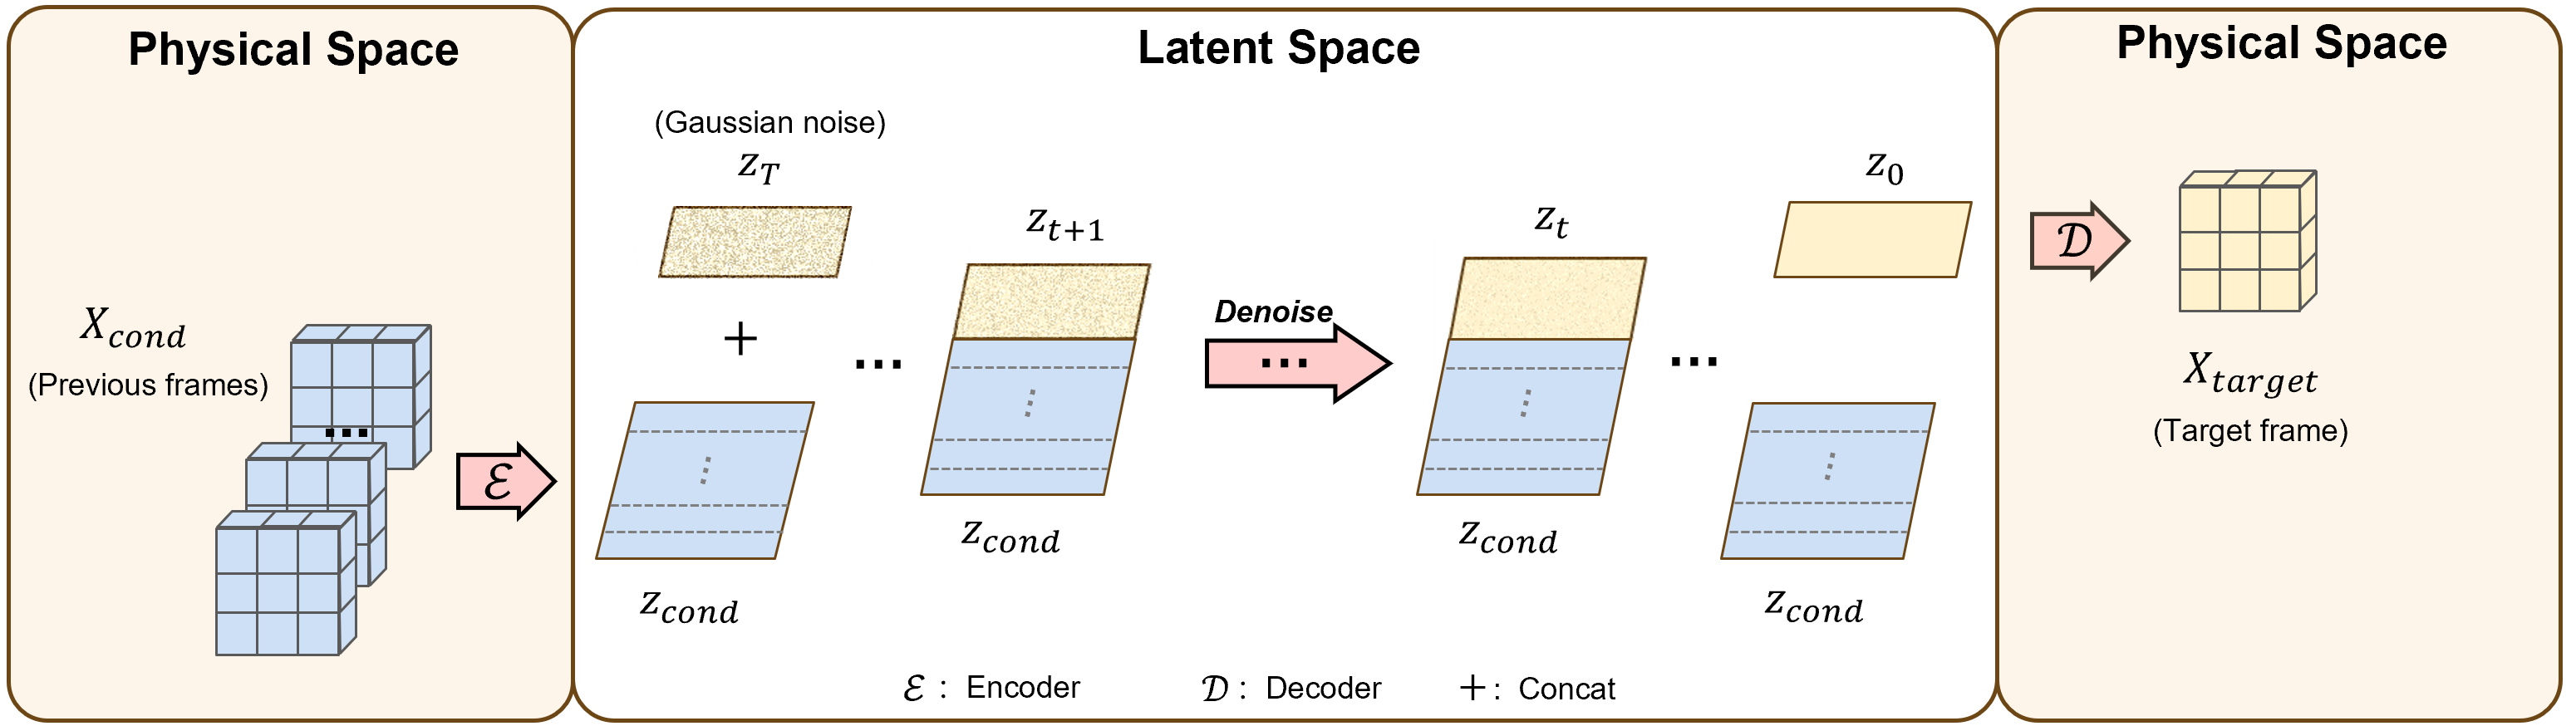
\includegraphics[width=16cm]{figures/workflow.png}
    \caption{Overview of the implemented Latent Diffusion system inference workflow.}
    \label{fig:workflow}
\end{figure}
%TC:endignore

\subsection{Reduced-order model: frame-wise convolutional autoencoder}
Reduced-order modelling typically involves dimensionality reduction methods, which are essential for handling the fine-grained 3D structural data generated by CFD simulations \cite{zuo2010fast, masoumi2022review}. In this work, a convolutional autoencoder (CAE) is implemented that serves a dual purpose: it acts as a dimensionality reduction technique and simultaneously learns meaningful latent embeddings for the use of the second-stage prediction model. The training of this CAE model adheres to the standard autoencoder training framework, where the objective is defined as a reconstruction task. By minimizing the reconstruction error, the CAE model not only learns to efficiently reconstruct the original data, but learns a meaningful encoder to compress the original data into lower dimensions. Besides, although the dataset used may contained temporal information of the whole domain at different time steps. The input and output of this CAE model are treated in a frame-wise manner without taking considering of temporal relationships between consecutive time steps. \\ 

\textbf{Training workflow}: As shown in Figure \ref{fig:cae_training_workflow}, the frame-wise CAE contains an encoder $\mathcal{E}$ and a decoder $\mathcal{D}$ that first encodes the training grid into a 1D latent space, and then reconstructed back to the physical space. Supposed that the input grids in a training batch at random time steps are given as:
$$
    X_n = [x_1, x_2, \cdots, x_n] \in \mathbb{R}^{C \times D \times H \times W}
$$
where $C$ is the number of different physical fields, and $D$, $H$, and $W$ denotes the spatial resolution of the whole grid. Then, the CAE first encodes $X_n$ into the 1D latent embedding $z_n \in \mathbb{R}^{latent\_dim}$ through the frame-wise encoder $\mathcal{E}$, and then the latent embedding $z_n$ is fed to the decoder $\mathcal{D}$ to decode back to the reconstructed grid $X^{'}_n$. The training objective is to minimize the L2 pixel-wise loss $\mathcal{L}(X_n, X^{'}_n)$ between the input grid $X_n$ and the reconstructed grid $X^{'}_n$. Details of this procedure can be formulated using the following equations:
\begin{align}
    z_n &= \mathcal{E}(X_n) \in \mathbb{R}^{latent\_dim} \nonumber\\
    X^{'}_n &= \mathcal{D}(z_n) \in \mathbb{R}^{C \times D \times H \times W} \nonumber\\
    \mathcal{L}(X_n, X^{'}_n) &=  \mathbb{E}_{X_n}\left\|\mathcal{D}(\mathcal{E}(X_n)) - X_n\right\|^2_2
\end{align}
Therefore, turning to the spatial-temporal prediction problem, the input observation sequence $X_{cond} \in \mathbb{R}^{M \times C \times D \times H \times W}$ that contains $M$ consecutive time steps can be compressed by the trained frame-wise encoder $\mathcal{E}$ into the latent embeddings $z_{cond} \in \mathbb{R}^{M \times latent\_dim}$, which will be further fed into the second-stage prediction latent diffusion model.
%TC:ignore
\begin{figure}[htbp]
    \centering
    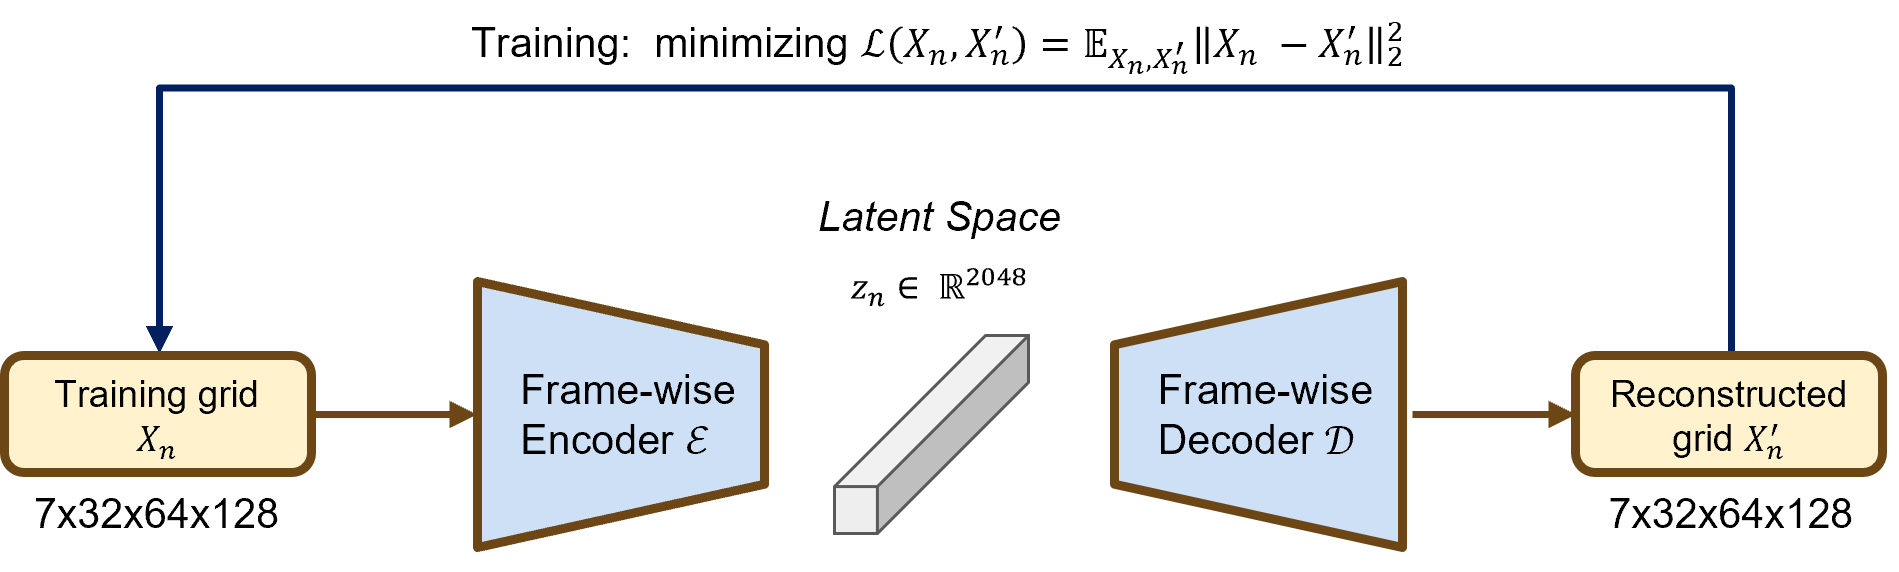
\includegraphics[width=15cm]{figures/cae_training_workflow.png}
    \caption{Frame-wise convolutional autoencoder training workflow.}
    \label{fig:cae_training_workflow}
\end{figure}
%TC:endignore

\textbf{Network design}: For the specific architecture of this CAE model (see Appendix \ref{fig:cae}), it contains an input projection Conv3d layer (4x4, stride 2), together with 4 ResNet-like residual blocks in the encoder $\mathcal{E}$. For each residual block, it has 2 Conv3d layers (3x3) using a combination of group norm and SiLU activation. Besides, a down-sampling Conv3d layer (4x4) with stride 2, is also used after each residual block to reduce the spatial resolution of the grid step by step by a factor of 2. Finally, the last layer of the encoder $\mathcal{E}$ is a fully-connected layer that projects the extracted feature map to 1D latent embeddings. Meanwhile, the design of the decoder $\mathcal{D}$ follows a similar up-sampling schedule, but with 5 residual-upsampling block pairs to ensure the reconstructed output has the same spatial resolution. For each upsampling block, it uses a combination of a Upsampling layer with a Conv3d layer (3x3) to increase the spatial dimension by a factor of 2. Then, a final project Conv3d layer is used at the end of the decoder $\mathcal{D}$ to ensure the reconstructed output has the same number of channels (i.e., number of physical fields). 

\subsection{Conditional latent diffusion model}
\subsubsection{Preliminary: Denoising Diffusion Probablistic Model (DDPM)}
Denoising Diffusion Probablistic Models (DDPMs) are probablistic models that are trained to capture the input data distribution $p(x)$ through a discrete process of reversing the noise added to the data \cite{yang2024survey, ho2006diff}. Typically, a DDPM consists of a forward diffusion process and a backward denoising process. In the diffusion process, Gaussian noise is added to the original data in discrete steps $t \in [1, 2, \dots, T]$ based on Markov chains, where the transition distribution in this process can be denoted as:
\begin{align}
    p\left(x_t \mid x_{t-1}\right) &= \mathcal{N}\left(x_t ; \sqrt{1-\beta_t} \cdot x_{t-1}, \beta_t \cdot \mathbf{I}\right) \nonumber\\
    p\left(x_t \mid x_0\right) &= \mathcal{N}\left(x_t ; \sqrt{\hat{\alpha_t}} \cdot x_0,\left(1-\hat{\alpha}_t\right) \cdot \mathbf{I}\right) \label{eq:alpha_t_cumprod}\\
    \alpha_t &= 1 - \beta_t \nonumber\\
    \hat{\alpha}_t &= \prod_{i=1}^{t} \alpha_i
\end{align}
where $T$ is the predefined total amount of diffusion steps, and $\beta_t$ denotes the variance schedule of noise added to the data from $t=1$ to $t=T$. The coefficient $\alpha_t$ is derived from $\beta_t$, and the cumulative product $\hat{\alpha_t}$ is crucial for determining the mean and variance of the Gaussian transitions in this process, as shown in Equation (\ref{eq:alpha_t_cumprod}) \cite{gao2024prediff}. The reason why such variance schedule is chosen is to approximately make $x_0$ follows the true data distribution $p(x)$ and $x_T$ follows the Gaussian noise $\mathcal{N}(0, I)$. Similarly, the reverse process parameterized by the DDPM should follow the same Gaussian transition as in the diffusion process for each step:
\begin{align}
    p\left(x_{t-1} \mid x_{t}\right) &= \mathcal{N}\left(x_{t-1} ;\mu_t(x_t, t), \beta_t(x_t, t)\right) \label{eq:reverse_transition} \\
    p\left(x_{0: T}\right) &= p\left(x_T\right) \prod_{t=1}^T p\left(x_{t-1} \mid x_t\right)
    \label{eq:cumprod_reverse}
\end{align}

which indicates that one can follow (\ref{eq:reverse_transition}) to reverse from the Gaussian noise $x_T \sim \mathcal{N}(0, I)$ step by step to the true data distribution $x_0 \sim p(x)$ \cite{ho2006diff}. \\

% However, due to the nature of high dimensionality in fluid dynamics data, this process can be computationally intensive and challenging to accurately model directly. Thus, the problem of nowcasting indoor airflow dynamics can be formulated in the latent space using a Latent Diffusion Model (LDM) \cite{rombach2022highresolution}.

\subsubsection{Latent diffusion}
As stated in the original Latent Diffusion Model paper \cite{rombach2022highresolution}, the denoising backbone network can be conditioned to guide and control the generation results of the denoising process, and the condition can be results of any upstream tasks such as text, images, or any latent embeddings. Therefore, following section \ref{meth:overview}, this problem can be formulated as a spatial-temporal prediction problem, and a classic DDPM in the latent space can be constructed to parameterize the latent conditional distribution $p(z_{0:T} | z_{cond})$ based on Equation (\ref{eq:cumprod_reverse}):
\begin{equation}
    p\left(z_{0: T}\right|z_{cond}) = p\left(z_T\right) \prod_{t=1}^T p\left(z_{t-1} \mid z_t, z_{cond}\right)
\end{equation}
where $z_{cond} \in \mathbb{R}^{latent\_dim}$, is a one-dimensional latent vector of the input previous-step sequence, encoded by the frame-wise encoder $\mathcal{E}$. Given this latent embedding $z_{cond}$, the denoising process can be started from Gaussian noise $z_T \sim \mathcal{N}(0, \mathbf{I})$, to the true data distribution $z_0 \sim p(z | z_{cond})$. This indicates that during inference, the spatial-temporal prediction problem can be transformed into a conditional generation problem in the latent space as long as the latent embedding $z_{cond}$ is given. And finally, through the frame-wise decoder $\mathcal{D}$, the predicted latent embedding of future frames can be then decoded back to the physical space. \\

\textbf{Training workflow}: During the training process, instead of directly predicting over the latent embedding $z_{t-1}$, an alternative way is to train the model to learn the noise $\epsilon_t$ transited at each time step $t$ \cite{rombach2022highresolution, gao2024prediff}. Specifically, as illustrated in Figure \ref{fig:ldm_training}, when starting with a latent target sequence $z_0$, Gaussian noise is added in the forward diffusion process over each time step $t \in [1, T]$. Then, the Sinusoidal Positional Encoding method, which has been widely used in Transformer architectures \cite{vaswani2017attention}, is adopted to incorporate the positional information of each diffusion time step $t$ into the network. The details of sinusoidal positional encoding involves mapping a temporal position onto a sin wave, where for a given scalar $t$, it is encoded into a vector $PE(t)$ via:
\begin{align}
    &PE(t)_{2i} = \sin (\frac{t}{10000^{2i/d}}) \nonumber\\
    &PE(t)_{2i+1} = \cos (\frac{t}{10000^{2i/d}})
\end{align}
where $i$ represents the dimension index in $PE$ and $d$ is the dimension size. In this way, each discrete time step $t$ can be encoded to a time embedding $\mathbf{t}$ to represent the temporal information of the diffusion sequence. Each time embedding $\mathbf{t}$ is then mapped by several MLP layers in order to be consistent with the dimensionality of the latent vector $z_t$. Then, for each time step $t$, the model is trained to predict the transition noise $\epsilon_t(z_t, \mathbf{t}, z_{cond})$ via maximum likelihood estimation over the L2 loss $\mathcal{J}_{LDM}$ of the transition noise:
\begin{equation}
    \mathcal{J}_{LDM}=\mathbb{E}_{(z_{cond}, z_t)}\left\|\epsilon-\epsilon_t\left(z_t, \mathbf{t}, z_{\text {cond }}\right)\right\|^2_2
\end{equation}
where $z_t$ is a target sequence and $z_{cond}$ is an observation sequence. \\

%TC:ignore
\begin{figure}[htbp]
    \centering
    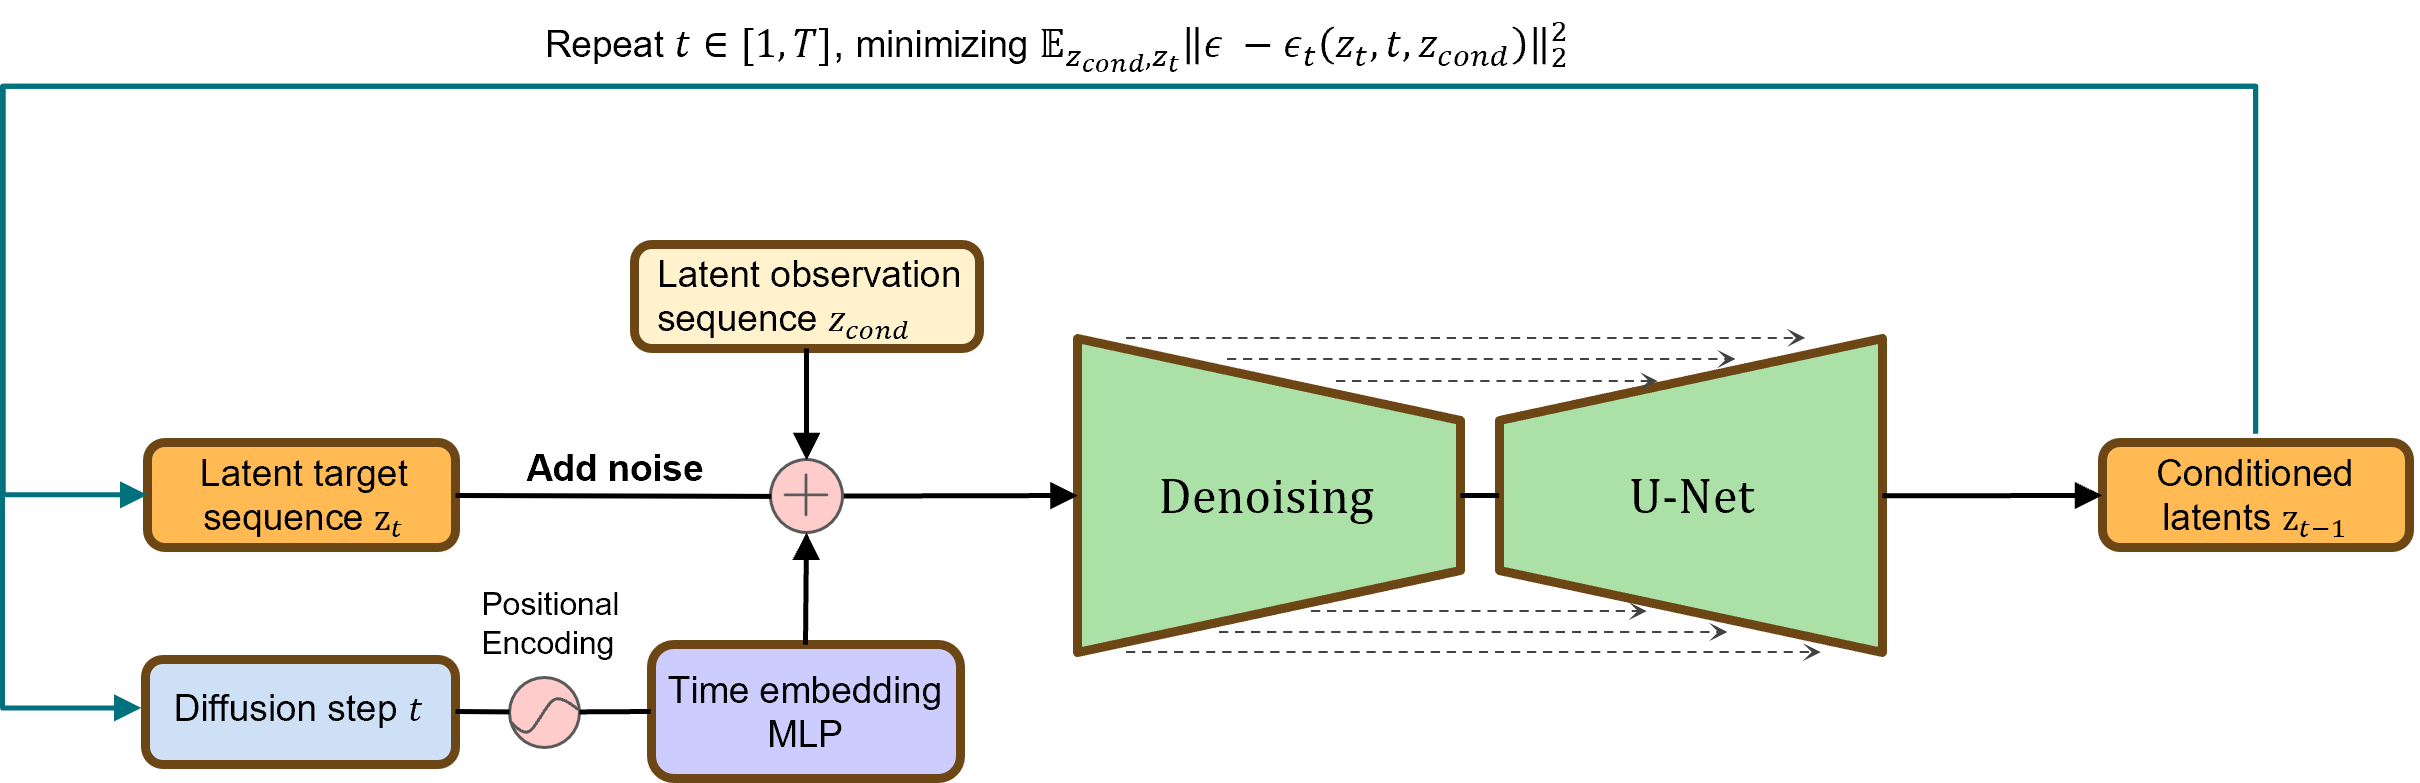
\includegraphics[width=16cm]{figures/ldm_training.png}
    \caption{Latent Diffusion Model training workflow.}
    \label{fig:ldm_training}
\end{figure}
%TC:endignore

\textbf{Network design}: As for the backbone network (see Appendix \ref{fig:unet}), I used a similar but simpler UNet architecture as the one in \cite{rombach2022highresolution}, while the vanilla attention is used in the bottleneck of my implementation rather than the original cross attention mechanism. Specifically, the Downsampling process contain 4 major modules, with each having 2 ResNet-like blocks \cite{he2016deep}, a Linear attention block, plus a projection downsampling layer, which is used to reduce the computational cost. For each ResNet block, it is made up of the combination of a 2D convolutional layer, group norm, and a SiLU activation. The time embedding mapped by the MLP layers are added in each Downsampling block to incorporate temporal information of the diffusion process. Similarly, the Upsampling blocks mimics the same schedule as in the Downsampling process, with the difference that residual connections are established between each downsampling and upsampling block, which is commonly adopted in UNet architectures. For the input of this network, the observation sequence $z_{cond}$ and the target sequence $z_{target}$ are just concatenated together before fed into the UNet. Notably, since both $z_{cond}$ and $z_{target}$ are 1D latent embeddings with dimensionality of $(\text{batch}, \text{seq\_len}, \text{latent\_dim})$, I rearranged it into $(\text{batch}, 1, \text{seq\_len}, \text{latent\_dim})$ in order to perform 2D convolution over the time axis.\\  




%%%%%%%%%%%%%%%%%%%%%%%%%%%%% Experiments and Results %%%%%%%%%%%%%%%%%%%%%%%%%%%%%%%%%%
\section{Experiments and Results}
\subsection{Experiment setup}
\subsubsection{Dataset description}
The dataset involved in this project consists of the full 3D simulations of a lecture room located at Houndsfield Primary School in London (Figure \ref{fig:classroom_schema}), generated by the AI4PDE method \cite{chen2024using}. The simulation models a typical classroom scenario where a teacher is instructing and students are seated around 4 desks. Besides, there is a people in the room moving back and forth within the room, allowing for the investigation of airflow dynamics under realistic, variable conditions. The data contains a total simulation time of $5000s$ of the airflow dynamics within the room, which means 500 time steps in total with a step size of $10s$. Each time step contains a snapshot of the whole mesh of 7 physical fields, which respectively are 'CO2 Tracer', 'Humidity', 'Pressure', 'Temperature', and the three components of the Velocity field: 'Vx', 'Vy', and 'Vz'. The original data has normalized the values of three fields with meaningful physical interpretations: 'CO2 Tracer,' 'Humidity,' and 'Temperature.' Therefore, to accurately restore these values to their respective physical scales, the field of 'CO2 Tracer' needs to be multiplied by a factor of $10^6$ to convert it to parts-per-million (ppm). Similarly, the field of 'Humidity' should be multiplied by 100 to represent it as percents, and the 'Temperature' field is .......... \\

%TC:ignore
\begin{figure}[htbp]
    \centering
    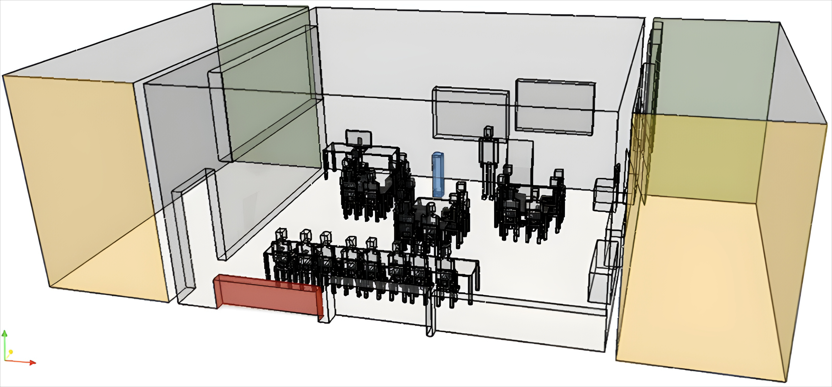
\includegraphics[width=13cm, trim=0.05cm 0.05cm 0.05cm 0.05cm, clip]{figures/classroom_schema.png}
    \caption{Schematic diagram of the classroom at Houndsfield Primary School, London.}
    \label{fig:classroom_schema}
\end{figure}
%TC:endignore

Regarding the spatial resolution, the original CFD data has a structural 3D mesh of $128 \times 256 \times 512$ data points. However, due to hardware constrains, the training data was downsampled by selecting every 4th point along each axis to alleviate computational cost, which results in a final spatial resolution of $32 \times 64 \times 128$ for each physical field in each snapshot.

\subsubsection{Data preprocessing}
The preprocessing procedure began with the downsampling of the original CFD data to obtain a spatial resolution of $32 \times 64 \times 128$, as mentioned above. Next, the values within the snapshot matrix for each physical field were examined and clipped to a physically plausible range to ensure consistency across the dataset, since there exist anomalously high values accumulated around the walls in fields such as 'CO2 Tracer', 'Humidity', and 'Temperature'. The dataset was then randomly divided into training and test sets in an 80:20 ratio. Subsequently, the snapshot matrices were normalized to the $[0, 1]$ range for numerical stability during the training of the first-stage frame-wise CAE. For the preprocessing required for training the diffusion model, the latent vectors encoded by the frame-wise CAE encoder were further scaled to the range between $[-1, 1]$, as typically a diffusion model expects.

\subsubsection{Hyperparameter configurations}
The specific configurations for training the CAE model and the latent diffusion model are detailed in Table \ref{tab:hyperparam}. Notably, the total diffusion steps for the diffusion model is chosen as 1000, and a linear beta schedule of $[0.0001, 0.02]$ is selected based on the results and implementation of \cite{ho2006diff, rombach2022highresolution} to achieve a stable and reasonable forward schedule. 

%TC:ignore
\begin{table}[ht]
    \centering
    \caption{Hyperparameter configurations of the CAE and the Latent Diffusion Model.}
    \tabcolsep=0.38cm
    \renewcommand\arraystretch{0.7}
    \scalebox{1}{
        \begin{tabular}[t]{lcc}
            \toprule
              & \multicolumn{1}{c}{\textbf{Hyperparameter Configurations}}\\
              \addlinespace
              & \textbf{CAE} & \textbf{LDM}\\
            \midrule
            Number of epochs & 200 & 50 \\
            Batch size & 32 & 32 \\
            Optimizer & Adam & Adam \\
            Learning rate & 5e-4 & 1e-4 \\
            Latent space dim & 2048 & - \\
            Diffusion steps & - & 1000 \\
            $\mathbf{\beta}$ schedule & - & $[0.0001, 0.02]$ \\
            \bottomrule
        \end{tabular}}
    \label{tab:hyperparam}
\end{table}
%TC:endignore

As for the running environment, the system is tested on Python 3.11 with PyTorch 2.3.1 accelerated by NVIDIA CUDA 12.1. Both the CAE and the LDM is trained on the Imperial HPC cluster. The hardware requested included two NVIDIA Quadro RTX 6000 GPUs and four AMD EPYC 7742 CPUs, supported by approximately 32GB of RAM. The training time of the CAE compression model requires around 30 minutes, while the diffusion model takes approximately 10 minutes under such configuration.
 

\subsection{Results and discussion}
\subsubsection{First stage: CAE reconstruction performance}
Based on the findings by Rombach \textit{et al.} \cite{rombach2022highresolution} and Gao \textit{et al.} \cite{gao2024prediff}, the performance of the Latent Diffusion model is highly dependent on the autoencoder trained in the first stage. Therefore, it is crucial to evaluate the effectiveness of the first-stage autoencoder's ability to compress the grid of high dimensionality into a meaningful latent space and accurately captures the underlying physical dynamics when reconstructing back to the original data. The CAE was configured with a latent size of 2048, which achieved a compression ratio of approximately 896 ($7 \times 32 \times 64 \times 128 / 2048$). Then, the CAE's reconstruction performance was assessed in terms of four fields 'CO2 Tracer', 'Temperature', 'Vx', and 'Vy'. These results were examined and presented as xy-slices at a height corresponding to z\_idx=16, at time points of $t = 1500s, 3000s, 4500s$ respectively. The former two time points are from the training set while the data at $t = 4500s$ were drawn from the unseen data.\\

As illustrated in Figure. \ref{fig:cae_recon_results}, the result indicates that the CAE model can effectively captures the board physical patterns of the airflow dynamics across different time levels for each physical field in interest. The model also demonstrates similar performance over the unseen data. However, there is noticeable information loss before and after the reconstruction, where the model struggles to capture the nuances of the physical characteristics of the airflow dynamics. When finer details of the spatial variations are required, the model tends to confuse between different subtle nuances and leads to coarser reconstructions.
%TC:ignore
\begin{figure}[!htb]
    \centering
    \begin{subfigure}[t]{0.49\textwidth}
        \centering
        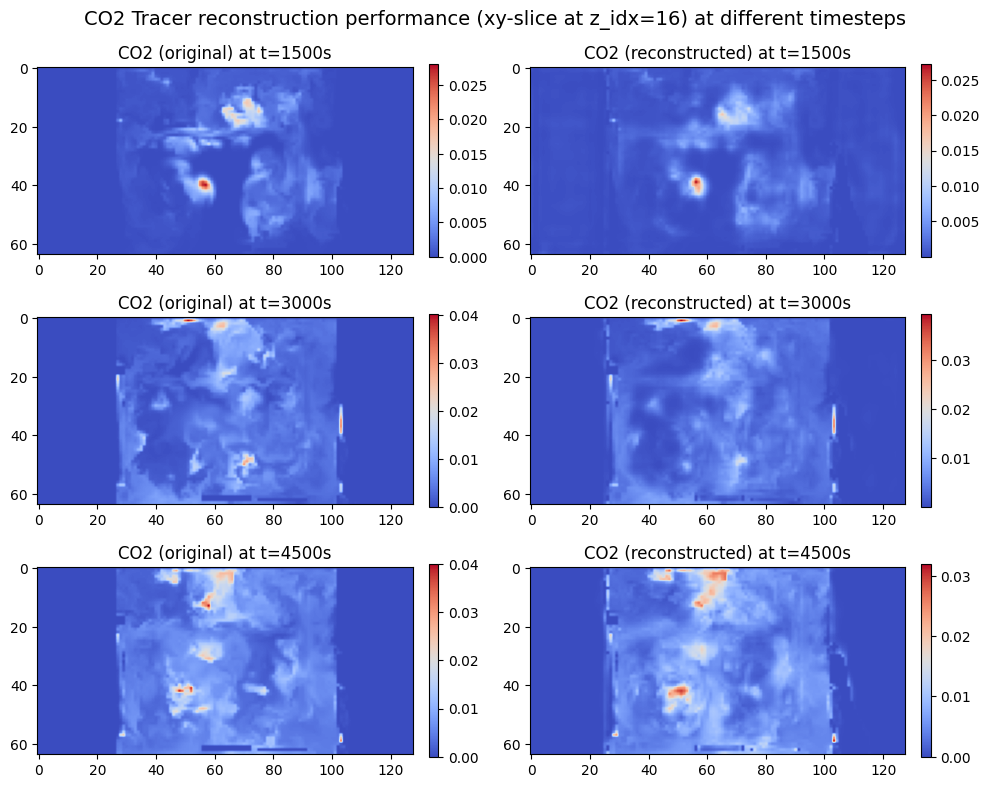
\includegraphics[width=\textwidth, trim=0cm 0cm 0cm 1cm, clip]{figures/co2_recon.png}
        \caption{CO2 tracer reconstruction.}
        \label{fig:co2_recon}
    \end{subfigure} \
    \begin{subfigure}[t]{0.49\textwidth}
        \centering
        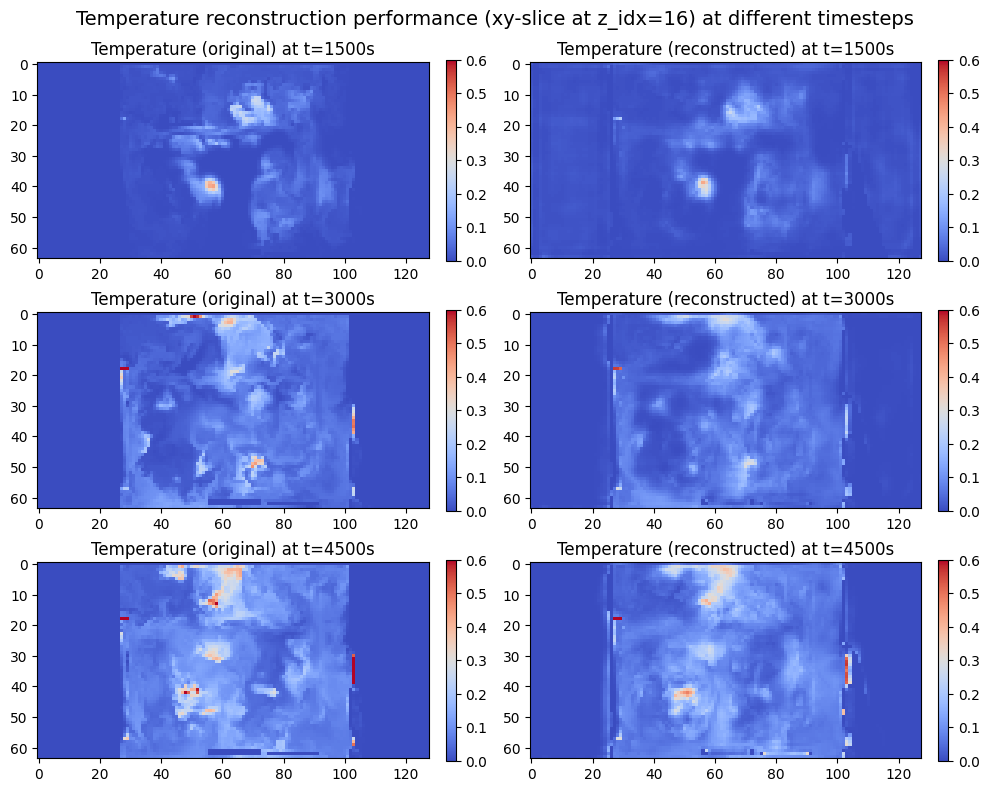
\includegraphics[width=\textwidth, trim=0cm 0cm 0cm 1cm, clip]{figures/temp_recon.png}
        \caption{Temperature reconstruction.}
        \label{fig:temp_recon}
    \end{subfigure} \\[5mm]
    \begin{subfigure}[t]{0.49\textwidth}
        \centering
        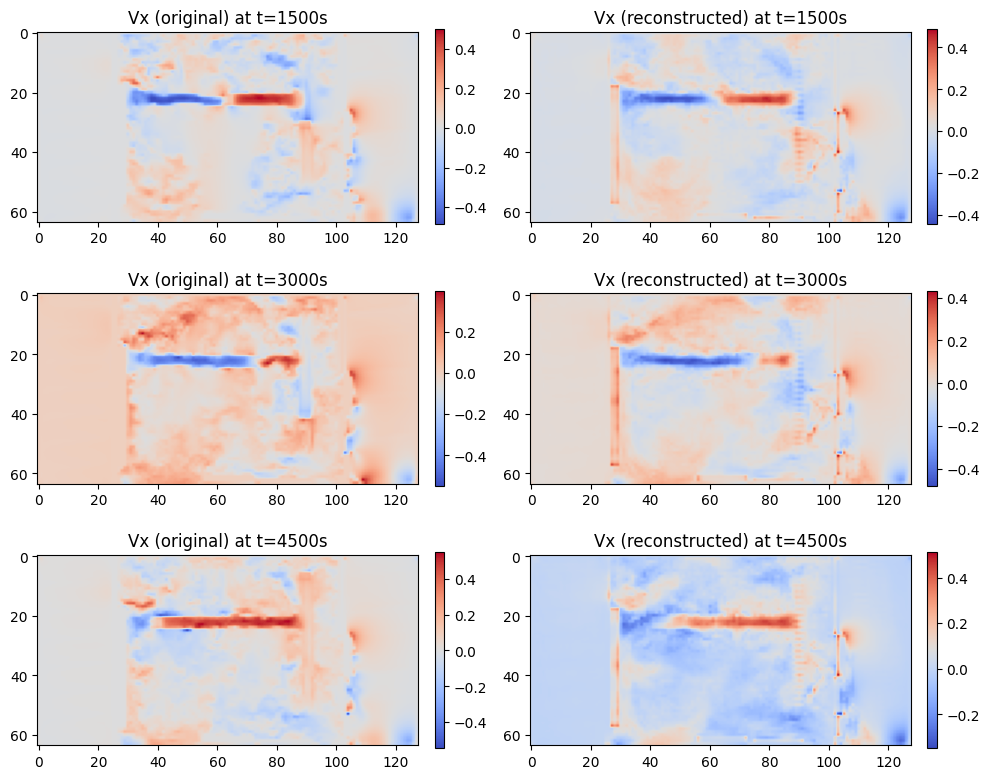
\includegraphics[width=\textwidth]{figures/vx_recon.png}
        \caption{Vx reconstruction.}
        \label{fig:vx_recon}
    \end{subfigure} \
        \begin{subfigure}[t]{0.49\textwidth}
        \centering
        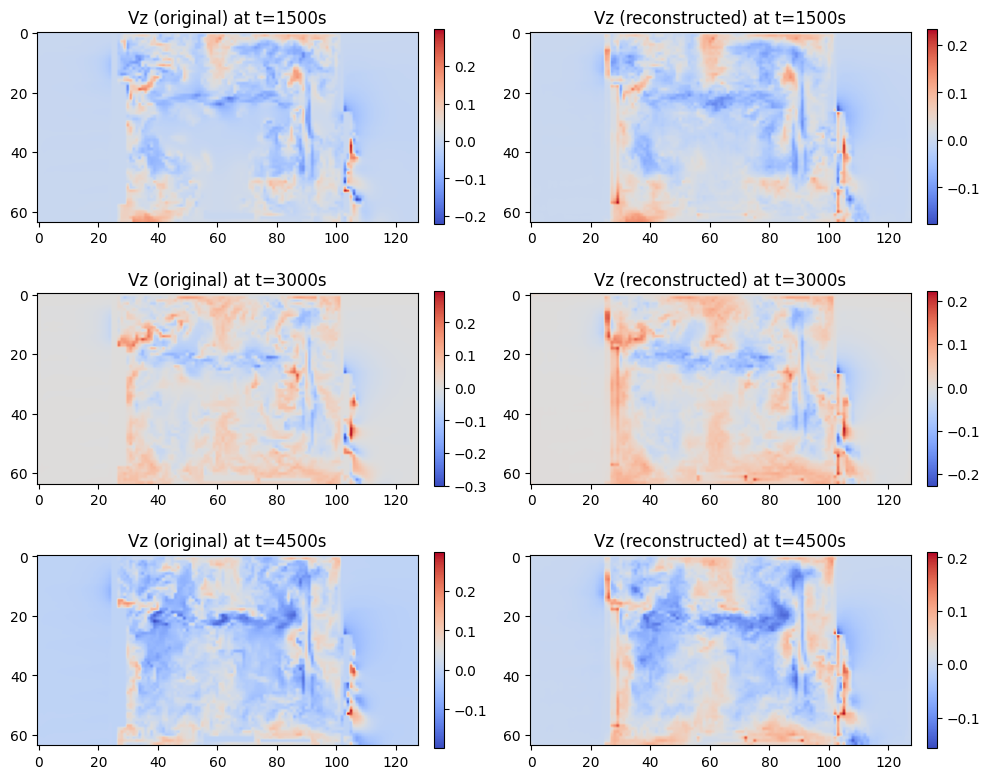
\includegraphics[width=\textwidth]{figures/vz_recon.png}
        \caption{Vz reconstruction.}
        \label{fig:vz_recon}
    \end{subfigure} \\
    \caption{Reconstruction results of xy-slice at z\_idx=16 for the fields 'CO2', 'Temperature', 'Vx', and 'Vz', at $t=[1500s, 2500s, 4500s]$  by using the implemented Convolutional AutoEncoder (CAE) to compress and reconstruct data respectively.}
    \label{fig:cae_recon_results}
\end{figure}
%TC:endignore


\subsubsection{Second stage: LDM prediction performance}
\textbf{Predicting for the training set:} After the first-stage model was trained, the full 3D grid data was encoded into 1D latent vectors using the encoder $\mathcal{E}$, and scaled to the range $[-1, 1]$ via Min-Max scaling. The diffusion model was then trained on the concatenated sequences of these latent vectors, where the previous 15 frames were used to predict the next one. This choice is due to the tiny changes between consecutive time steps in the original data, although the sequence length can be flexibly adjusted based on the specific characteristics of different datasets. As shown in Figure. \ref{fig:preds_latent}, the model's performance was examined at the time step $t = 2500$s, where the data between $[2500s, 2640s]$ correspond to the observed 15 frames, and then rolling-out predictions was conducted to autoregressively predict the next 10 frames of latent vectors. The prediction results in the latent space has demonstrated the LDM's ability to capture the temporal dynamics within the latent vectors, and can effectively generate predictions that are close to ground truth latent values.

%TC:ignore
\begin{figure}[!htb]
    \centering
    \begin{subfigure}[t]{\textwidth}
        \centering
        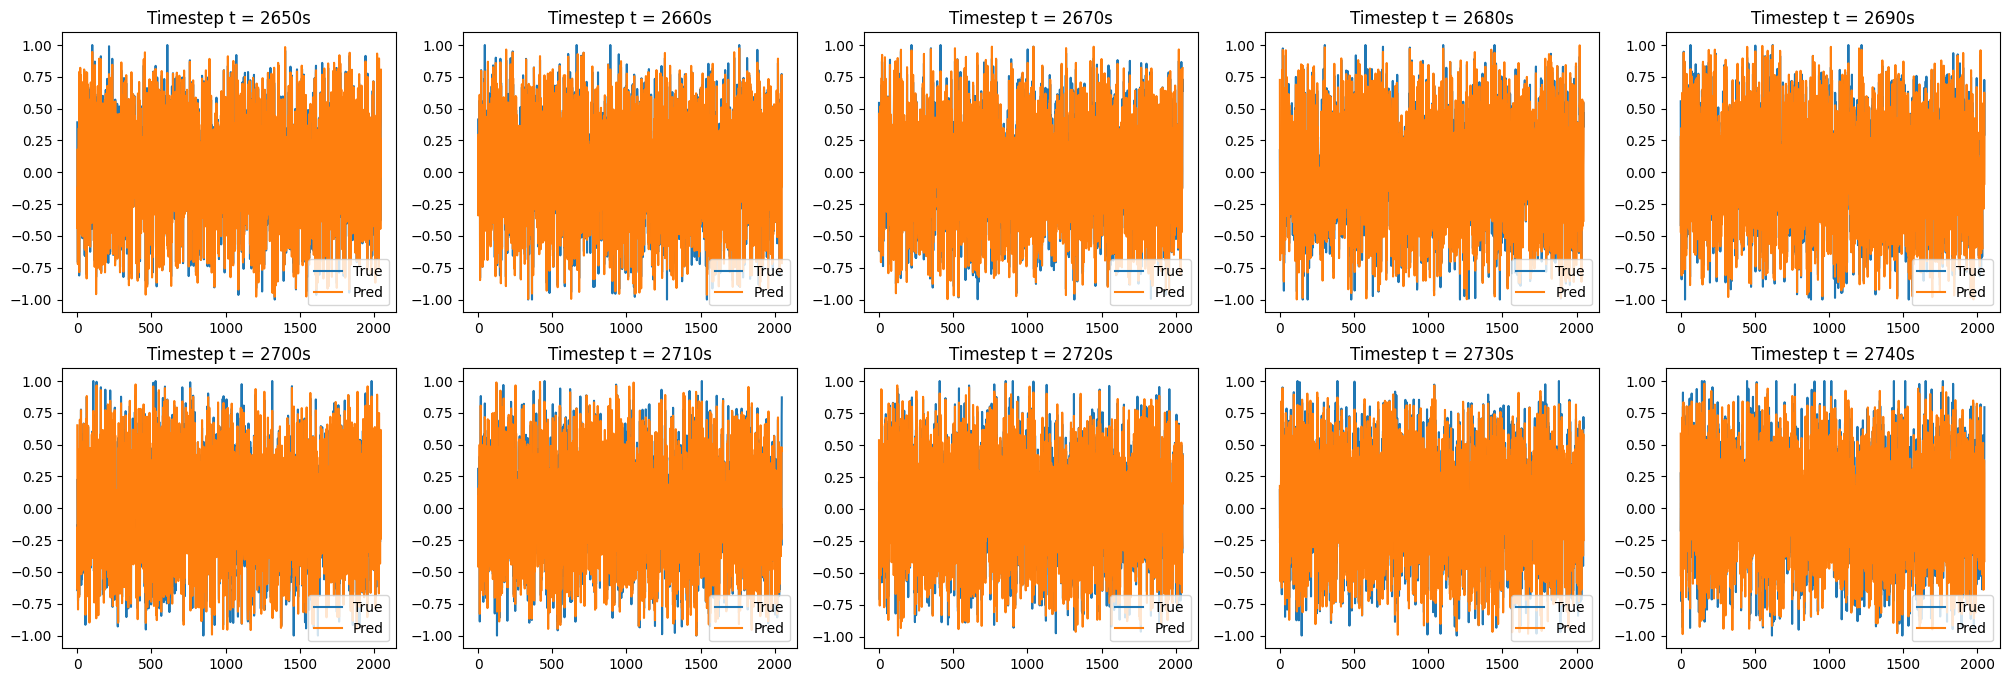
\includegraphics[width=\textwidth]{figures/latent_results.png}
        \caption{Prediction results of all 2048 dimensions of the latent vectors for the next 10 time steps.}
    \end{subfigure} \\[8mm]
    \begin{subfigure}[t]{0.7\textwidth}
        \centering
        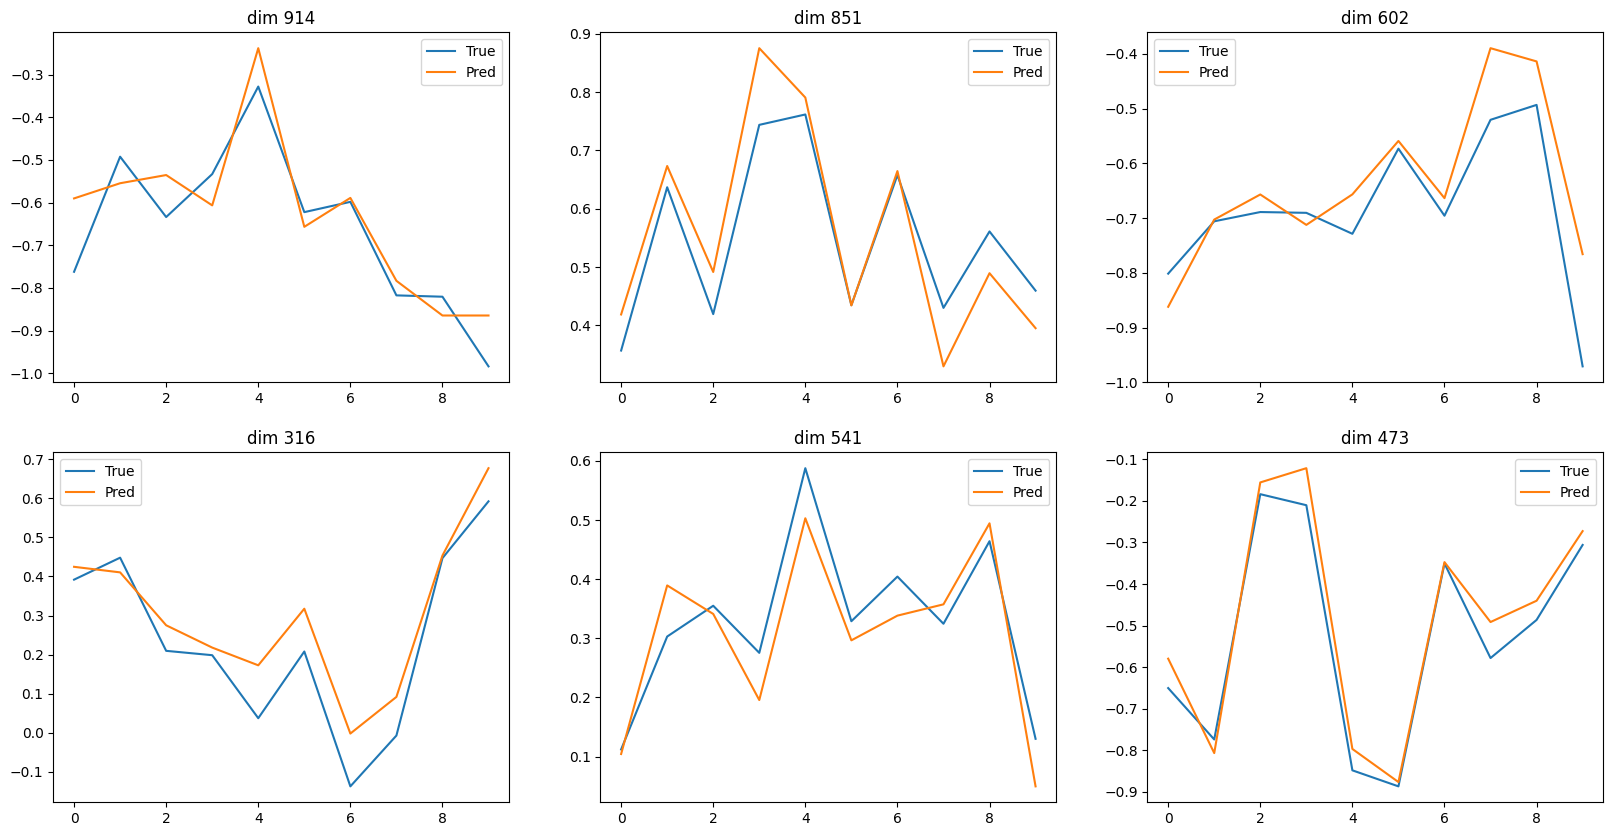
\includegraphics[width=\textwidth]{figures/latent_random_dim.png}
        \caption{Prediction results of the latent vectors evaluated at random dimensions for the next 10 time steps.}
    \end{subfigure} 
    \caption{Latent space predictions results using the LDM for the next 10 time steps where $t \in [2650s, 2740s]$.}
    \label{fig:preds_latent}
\end{figure}
%TC:endignore

Then, the predicted latent vectors were further decoded using the frame-wise decoder $\mathcal{D}$, to evaluate prediction performance in the physical space. Figure \ref{fig:pred_results_training} presents the predictions for the fields 'Temperature' and 'Vx' at $t \in [2650s, 2740s]$ in the training set for the next 10 time steps. Besides, prediction results of other fields at different slices can be found at Appendix \ref{fig:other_preds}, \ref{fig:other_preds_xy}. These results indicate that the latent diffusion model effectively learns meaningful temporal patterns within the fluid field. However, the results seem to have discrepancies in details compared to the ground truth, and some predictions may also violate physical laws, which may generate extremely high temperature values or irregular fluid patterns. We argue that these issues may stem from the limitations of the first-stage autoencoder, which was trained on a single case of the evolution of the indoor airflow, consisting of only 500 frames. Besides, the model was not regularized with any physical laws or guidance during training, which may also likely contribute to these unrealistic predictions. \\

%TC:ignore
\begin{figure}[!htb]
    \centering
    \begin{subfigure}[t]{0.99\textwidth}
        \centering
        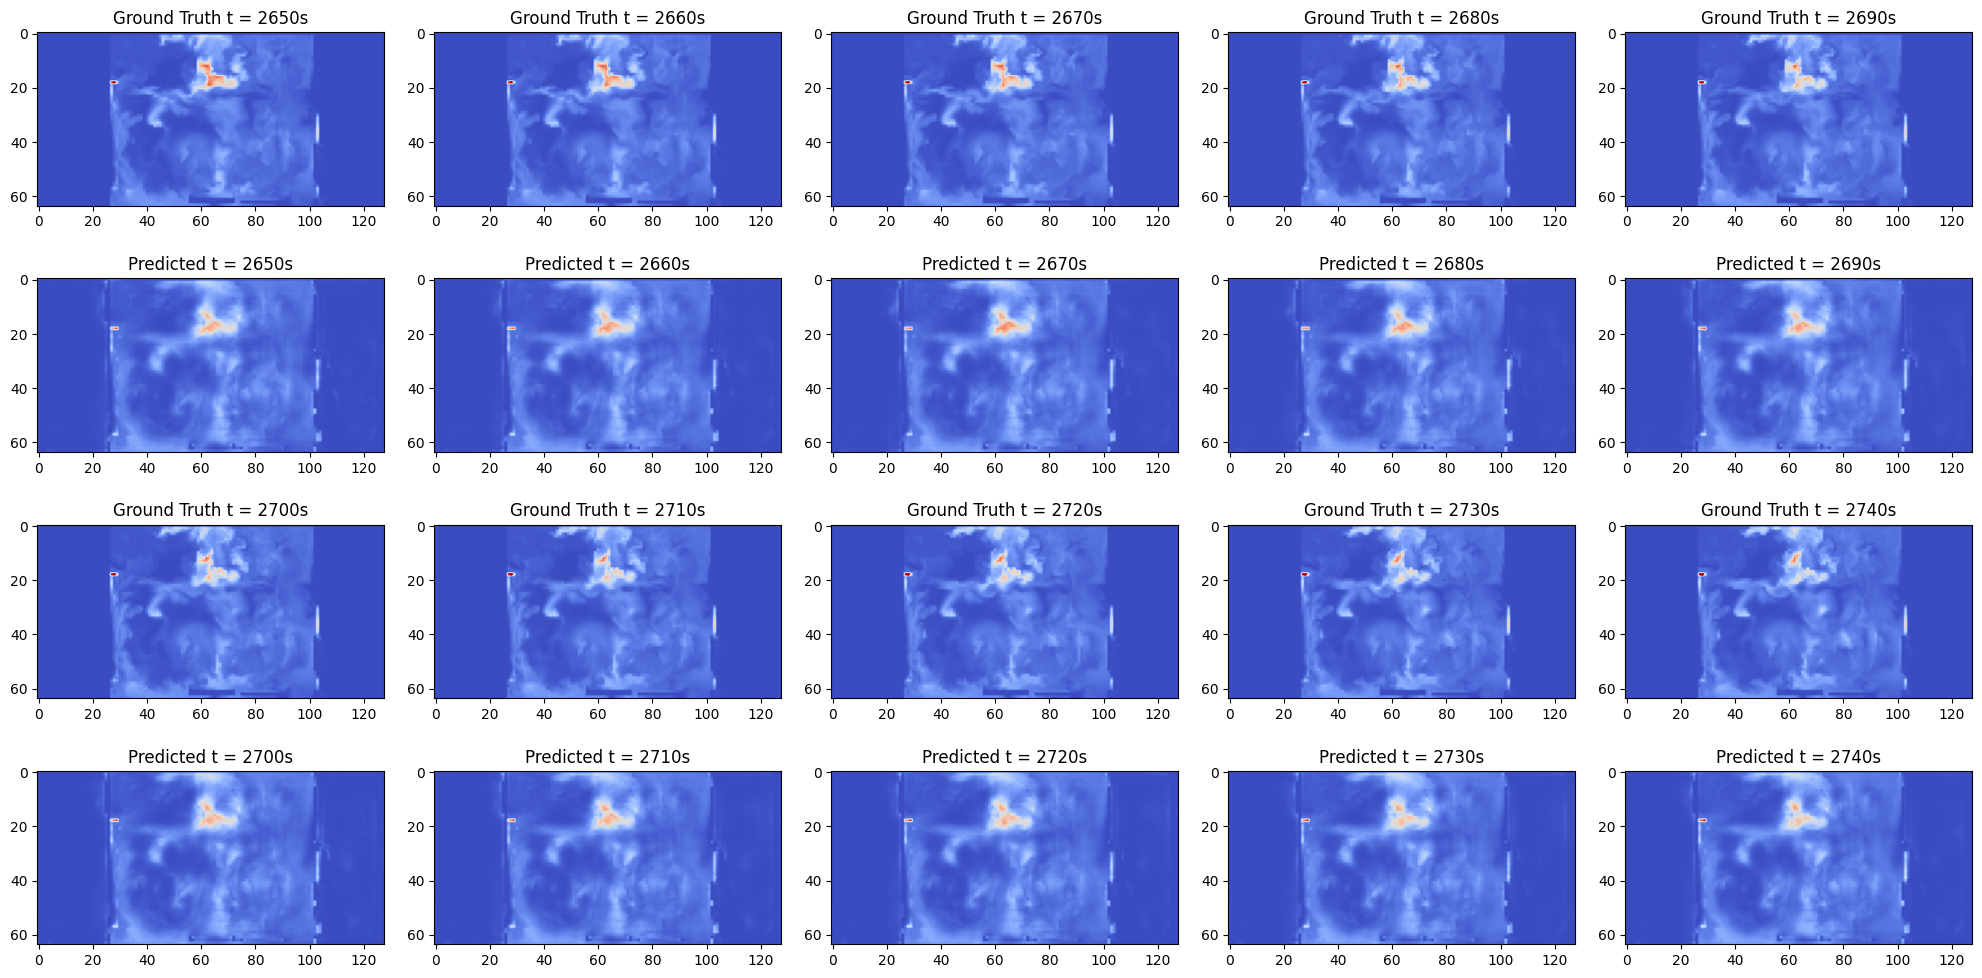
\includegraphics[width=\textwidth]{figures/temp_10_2650.png}
        \caption{Temperature predictions for the next 10 time steps $t \in [2650s, 2740s]$.}
    \end{subfigure} \\[8mm]
    \begin{subfigure}[t]{0.99\textwidth}
        \centering
        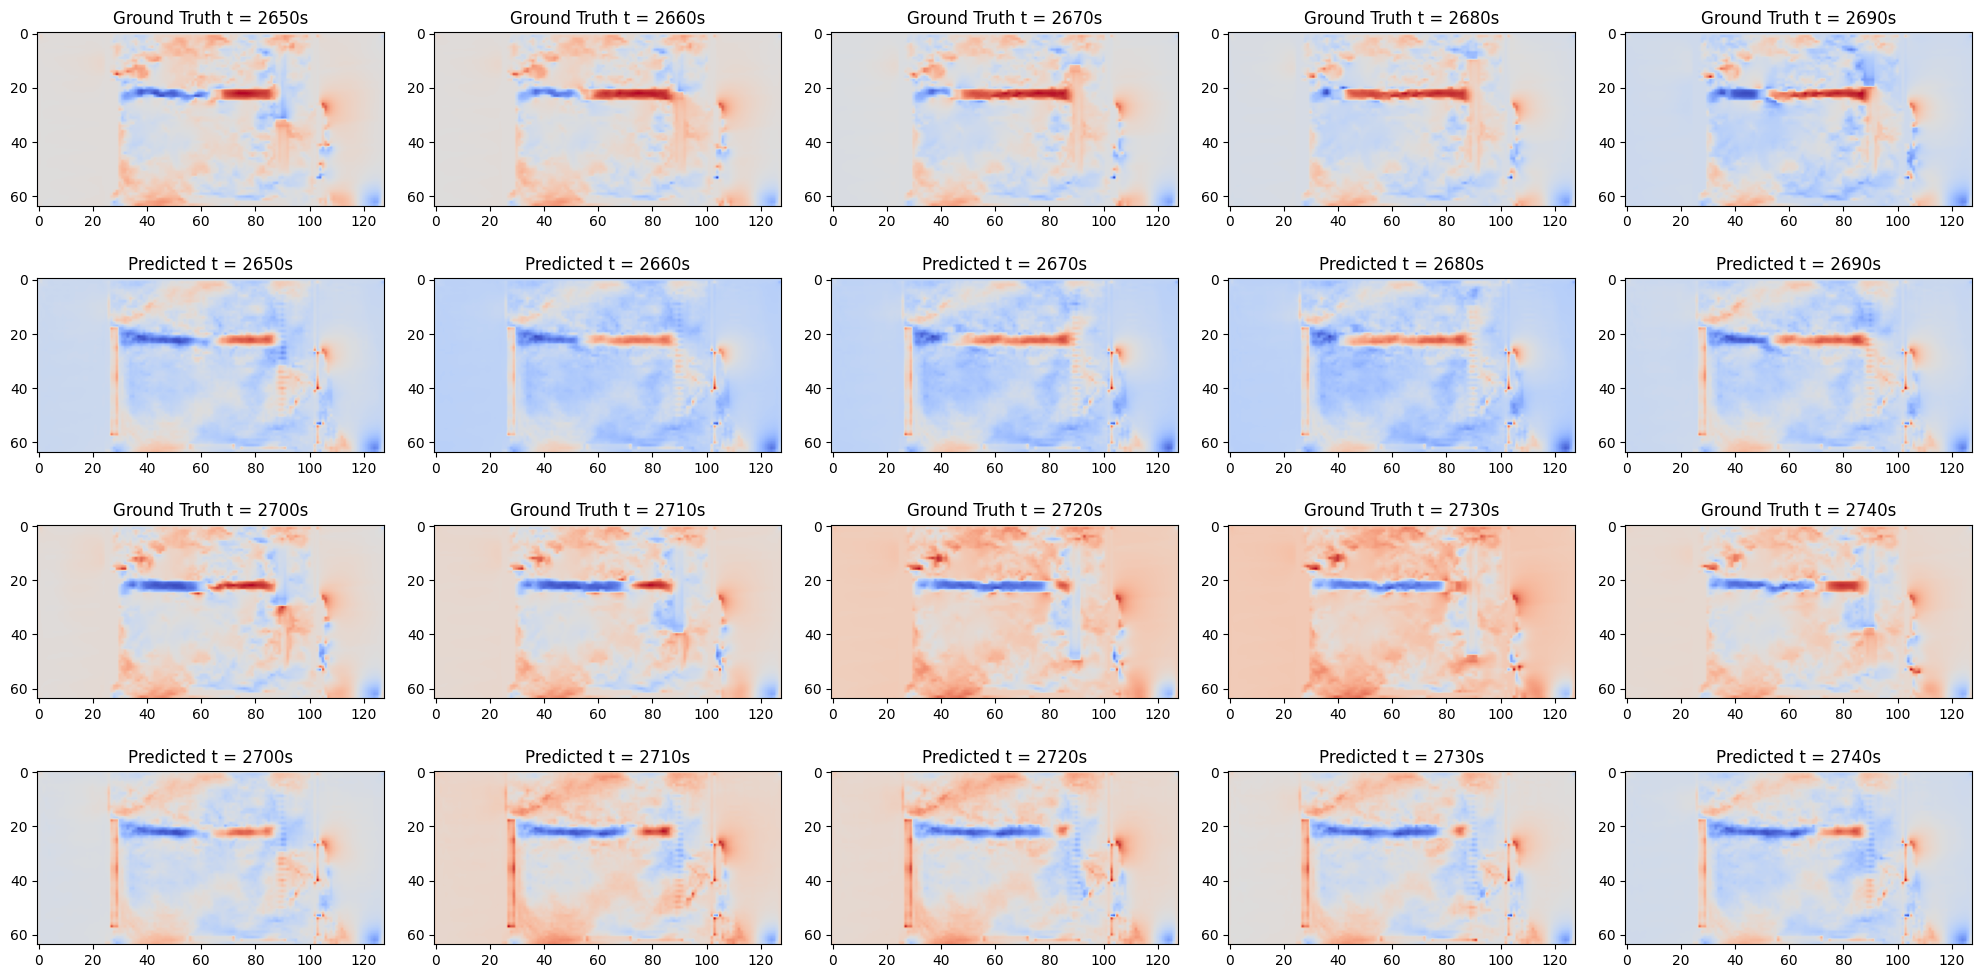
\includegraphics[width=\textwidth]{figures/vx_10_2650.png}
        \caption{Vx predictions for the next 10 time steps $t \in [2650s, 2740s]$.}
    \end{subfigure}
    \caption{Prediction results of xy-slice at z\_idx=16 for the fields 'Temperature' and 'Vx' for time step $t \in [2650s, 2740s]$ in the training set.}
    \label{fig:pred_results_training}
\end{figure}
%TC:endignore
\textbf{Predicting for the test set:} To further evaluate the model's capability over unseen data, we also evaluated the predictions at $t = 4200s$ in the test set, where the 15 time points between $[4200s, 4340s]$ served as the previous observed sequence used to condition the latent diffusion model. Figure \ref{fig:pred_results_test} illustrates the predictions for the next 10 frames at $t \in [4350s, 4440s]$ for the 'Temperature' and 'Vx' fields. The model shows good generalization ability on the test data consistent with the training set results, capable of capturing board spatial-temporal patterns of the airflow dynamics. For noticeable changes in the temperature field, see the hot spot emerging at the top of the figure through time (Figure \ref{fig:pred_results_test_temp}). 

%TC:ignore
\begin{figure}[!htb]
    \centering
    \begin{subfigure}[t]{\textwidth}
        \centering
        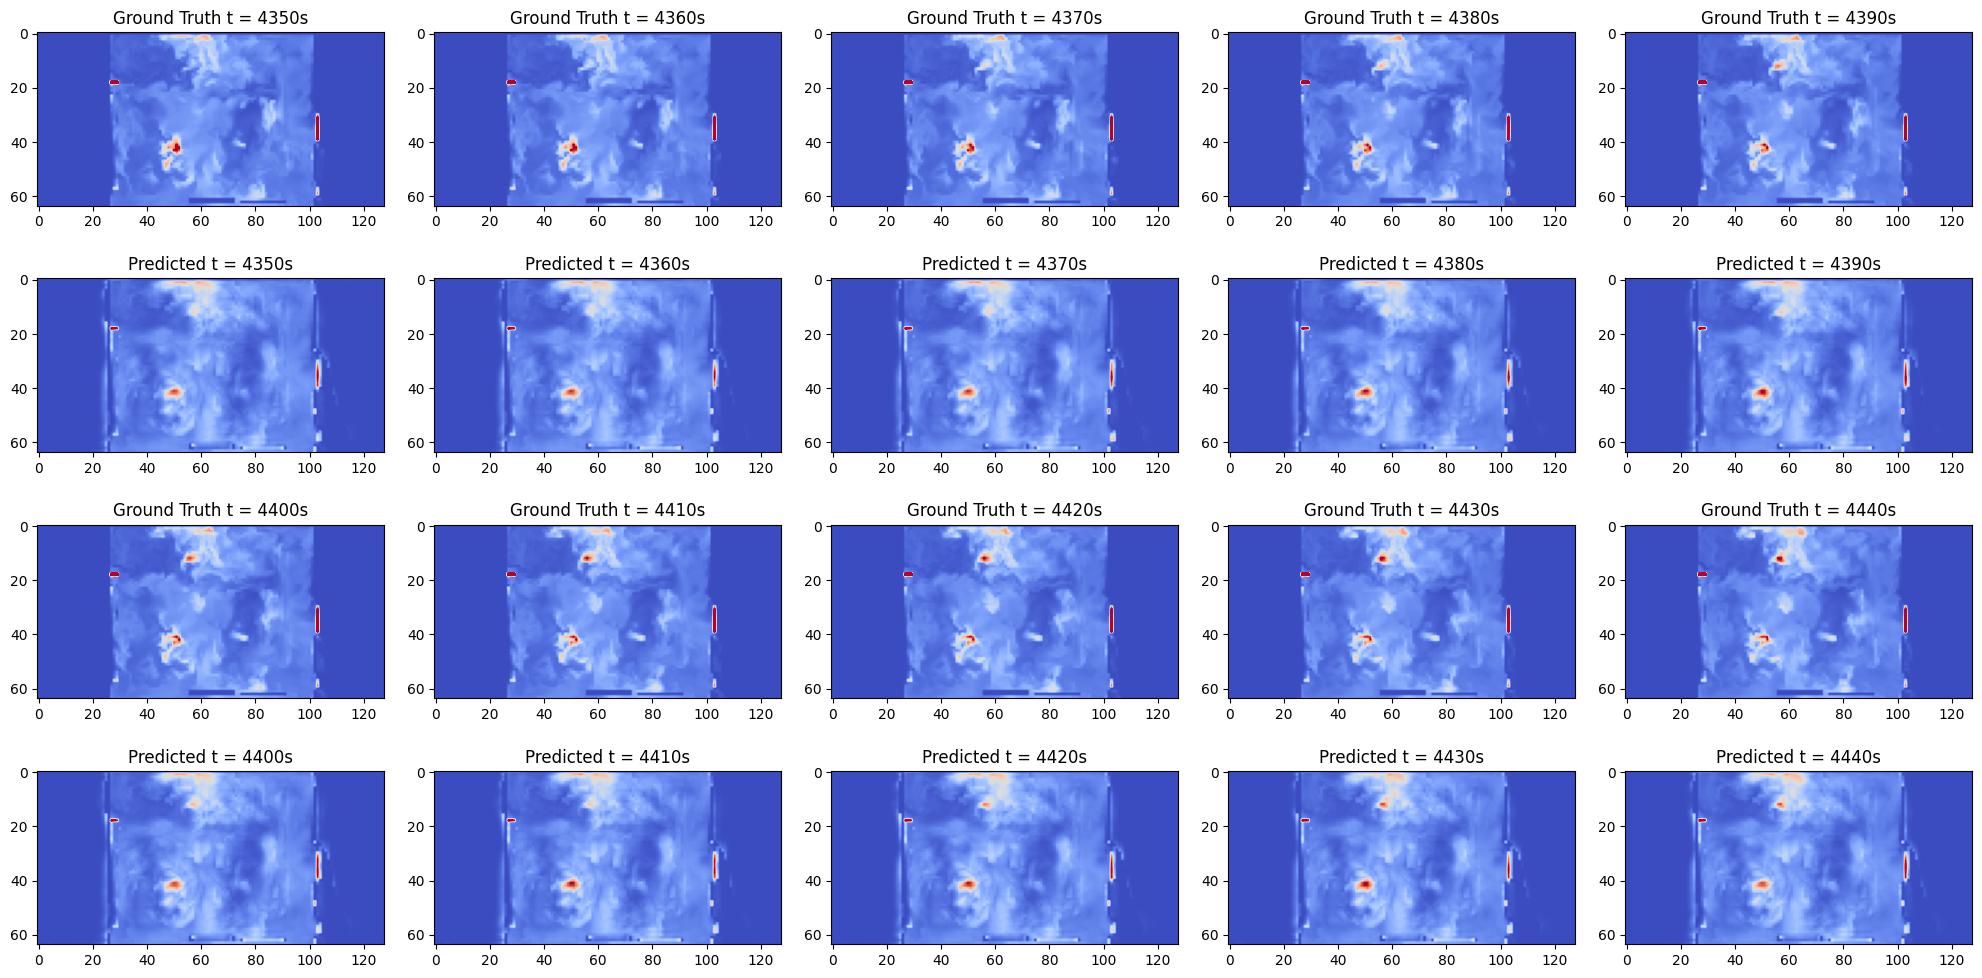
\includegraphics[width=\textwidth]{figures/temp_10_4350.png}
        \caption{Temperature predictions for the next 10 time steps $t \in [4350s, 4440s]$.}
        \label{fig:pred_results_test_temp}
    \end{subfigure} \\[8mm]
    \begin{subfigure}[t]{\textwidth}
        \centering
        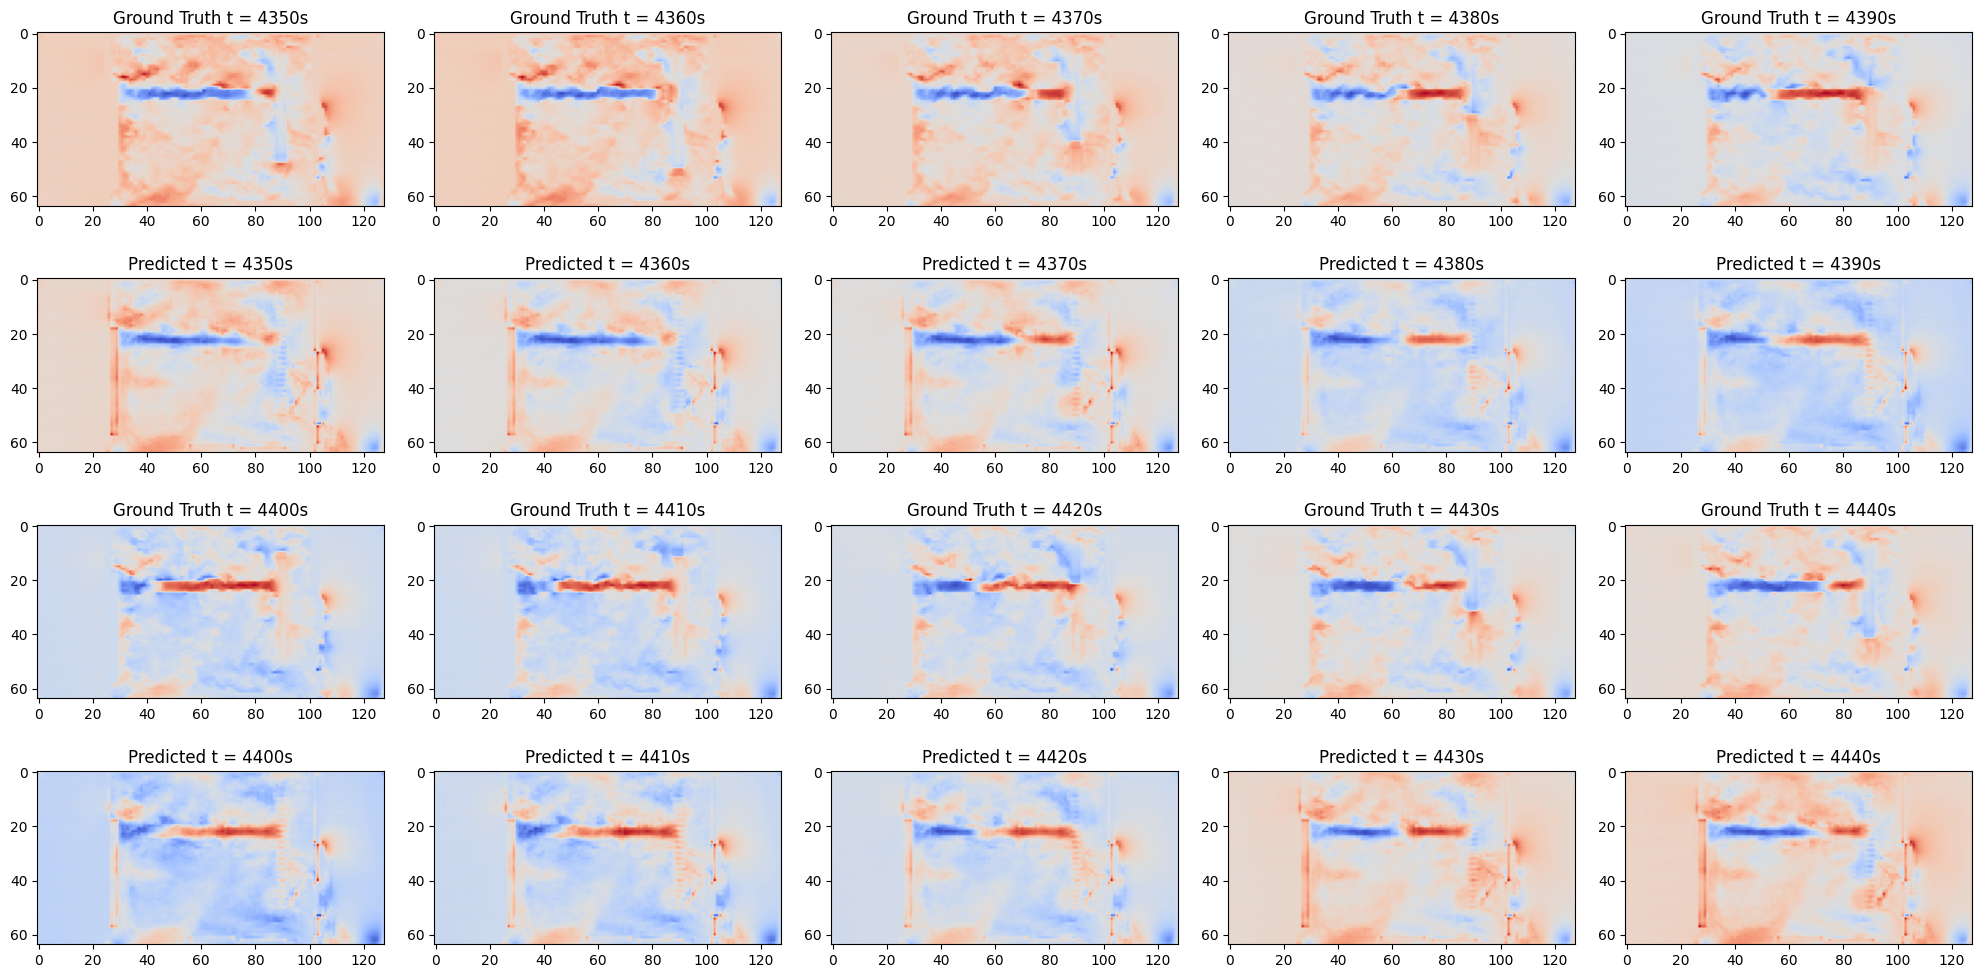
\includegraphics[width=\textwidth]{figures/vx_10_4350.png}
        \caption{Vx predictions for the next 10 time steps $t \in [4350s, 4440s]$}
    \end{subfigure}
    \caption{Prediction results of xy-slice at z\_idx=16 for the fields 'Temperature' and 'Vx' for time step $t \in [4350s, 4440s]$ in the test set.}
    \label{fig:pred_results_test}
\end{figure}
%TC:endignore

However, the results revealed similar issues to those observed in the training set that there were noticeable deviations from local nuances or expected physical behaviours. Additionally, when the test samples are away from the learned data distribution, such as the early stage of the airflow evolution, the model shows less capability to accurately generate predictions similar to the ground truth. Such limitations highlights the need of incorporating prior guidance or physical constraints during the model training \cite{gao2024prediff, bian2024diffusion}.\\

\textbf{Long-term predictions:} To examine the model's ability for long-term predictions as it is crucial for surrogate modeling, we performed the rolling-out prediction starting from $t = 2500s$ over the subsequent 100 time steps (equivalent to 1000s of simulation). Figure \ref{fig:pred_results_long_term} shows the model's predictions in both the latent space and the physical field 'Temperature': While the results are generally accurate in the short term for most dimensions, certain dimensions still exhibit deviations that will accumulate as the rolling-out prediction marches. This issue can be further exemplified in the physical space that the spatial variations will evolve differently in details in the long term compared with the ground truth due to these accumulated error in the latent space. We suspect the use of a 1D latent space of high dimensionality may damage the diffusion model's performance on accurately capturing the temporal relationships across all dimensions. However, since PyTorch currently does not support 4D convolutional layers to extract 3D feature maps within a time sequence, we still decided to use a 1D latent space in this implementation. Given more time, we would consider implementing 4D convolutions to potentially enhance the model's performance.

%TC:ignore
\begin{figure}[!htb]
    \centering
    \begin{subfigure}[t]{0.95\textwidth}
        \centering
        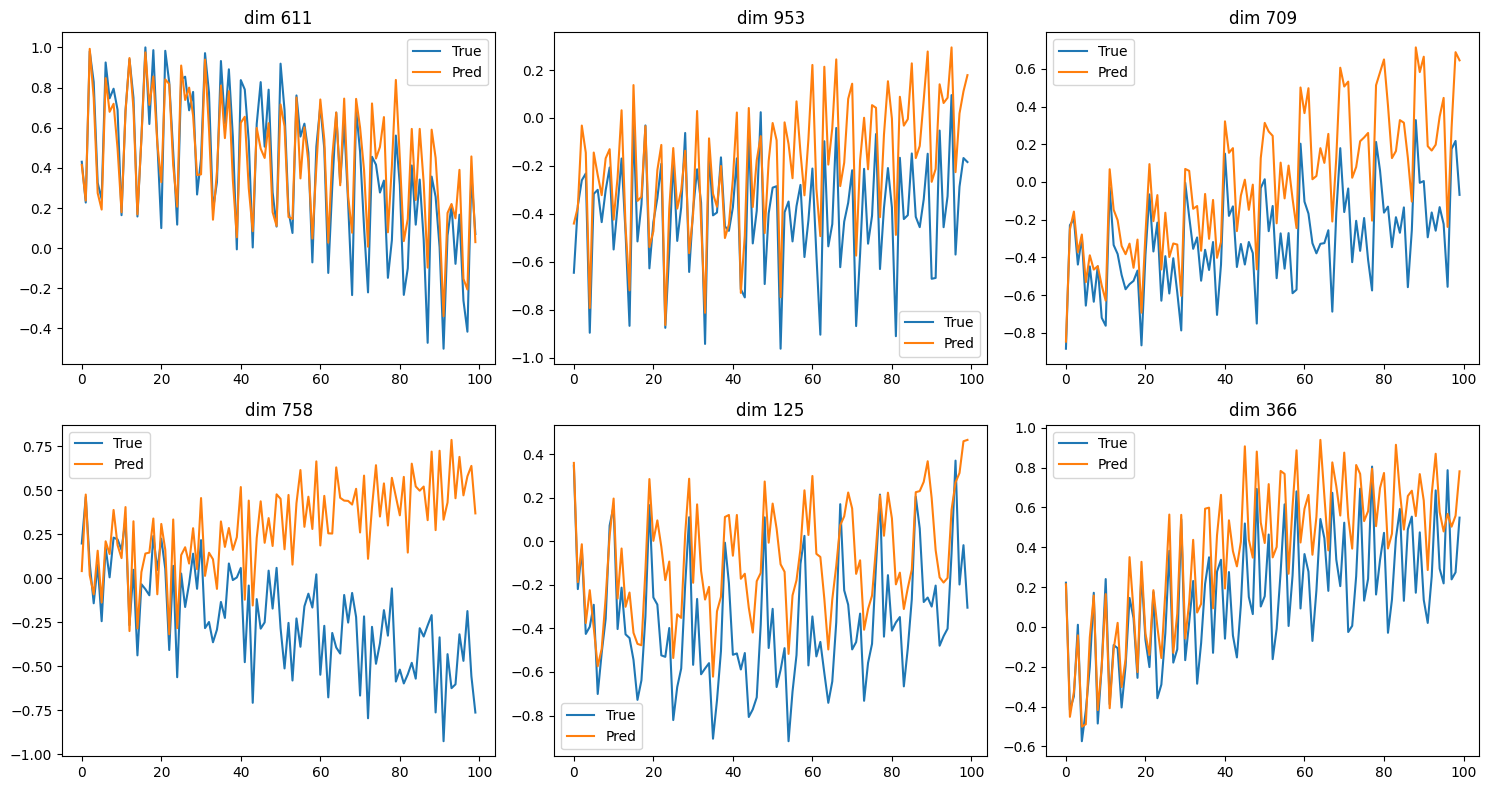
\includegraphics[width=\textwidth]{figures/long_term_100_latent.png}
        \caption{Predictions in the latent space for the next 100 time steps $t \in [2650s, 3650s)$, evaluated at random dimensions.}
    \end{subfigure} \\[8mm]
    \begin{subfigure}[t]{\textwidth}
        \centering
        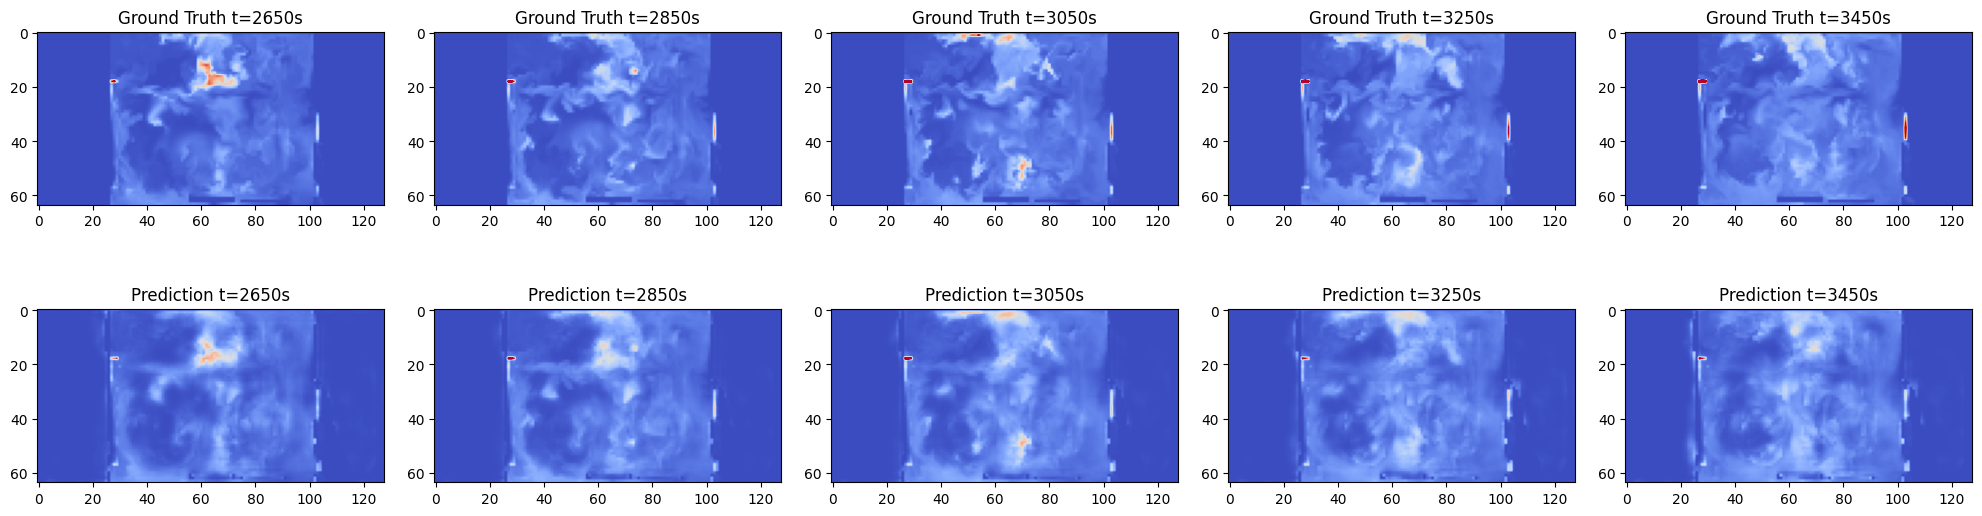
\includegraphics[width=\textwidth]{figures/long_term_100.png}
        \caption{Predictions of xy-slice at z\_idx=16 for the field 'Temperature' for time step $t \in [2650s, 3650s)$, sampled at every 200s.}
    \end{subfigure}
    \caption{Long term prediction results for the next 100 time steps $t \in [2650s, 3650s)$.}
    \label{fig:pred_results_long_term}
\end{figure}
%TC:endignore

% The expected results should be broadly in accordance with the established objectives in the following aspects:
% \begin{itemize}
%     \item The chosen ROM learns a meaningful representation of the input 3D CFD data in the latent space with significant reduction in dimensionality.
%     \item The LDM model is capable of producing realistic forecasts of the indoor airflow fields that have physical interpretations.
% \end{itemize}


% \begin{itemize}
%     \item Built up packaged code workflow on GitHub for reading, preprocessing, and visualize the 3D CFD data.
%     \item Implemented ROM models such as POD and a Convolutional Autoencoder to perform dimensionality reduction (see reconstruction results in Fig. ), as well as a PredAAE network for forecasting (see training results in Fig. ), similar to the one presented in Heaney's work \cite{heaney2024data}. Also, the data currently used is a subset of the classroom data in her research, only for testing the implemented framework.
%     \item Mostly finished reviewing related literature, and insights have been gleaned regarding the current state of research.
% \end{itemize}

\clearpage
% %TC:ignore
% \begin{figure}[htbp]
%     \centering
%     \includegraphics[width=16cm]{figures/PredAAE_recon_performance.png}
%     \caption{Reconstruction performance of the PredAAE model \cite{heaney2024data} in the latent space.}
%     \label{fig:predaae_recon}
% \end{figure}
% %TC:endignore

% \begin{itemize}
%     \item Continuously optimize the existing code workflow to accommodate new data, when CFD data from Direk's meeting room becomes available,
%     \item Retrain the ROM models using Direk's data, and explore alternative methods such as Variational Autoencoders.
%     \item Implement the Latent Diffusion Model for prediction of the airflow dynamics, with a thorough investigation into its architecture and time-series prediction techniques.
%     \item Establish multiple test cases and comparative experiments to verify implementation and uncover future insights.
%     \item Maintain the GitHub repository, leveraging GitHub Actions for automated testing.
%     \item Build documentation using Sphinx.
%     \item Complete the final dissertation write-up.
% \end{itemize}


%%%%%%%%%%%%%%%%%%%%%%%%%%%%%%%%%% Conclusion %%%%%%%%%%%%%%%%%%%%%%%%%%%%%%%%%%%%%%%%
\section{Conclusion, Limitation and Future Plan}
In this project, the author has designed a latent diffusion model for predicting the spatial variations of indoor airflow dynamics, and applied it to the simulations of a real classroom at Houndsfield Primary School, London. The model has demonstrated its potential of being adopted in surrogate modeling, which successfully captures the spatial-temporal relationship within the fluid dynamics, and allows to generate realistic predictions for various time steps ahead. It also shows a good generalization ability over unseen time steps in both latent space and decoded physical space.\\

However, the model also exhibits multiple limitations that lie on the following aspects, which needs to be further investigated if more time is given.\\

\textbf{Spatial discrepancies in nuances}: The model may suffer from capturing fine-grained spatial details compared with the original data. We suspect it may be due to the limitation of the first-stage autoencoder. Thus, further research can be conducted by replacing the 1D latent spaces with 3D feature maps, or resort to variational-based architectures such as the VAE or VQVAE \cite{van2017neural, rombach2022highresolution}. Besides, physical constraints may also need to be incorporated to regularize the autoencoder to generate more controllable results.\\ 

\textbf{Long term stability}: To fully apply this model into surrogate modeling, data assimilation techniques, such as 4D-Var, can be considered to guide the diffusion sampling and alleviate the rolling-out prediction error in the long term.\\  

\textbf{Ability to predict for other cases or geometries}: The model was currently trained and tested on a single airflow evolution scenario. To extend its applicability to different initial conditions, incorporating simulations from a broader set of cases into the training data is recommended, as suggested in \cite{yang2023denoising}. For predicting other geometries, domain decomposition methods can be considered to design the compression model in a scale-invariant manner when encountering larger spatial resolutions. 

%%%%%%%%%%%%%%%%%%%%%%%%%%%%%%%%%%%%% End %%%%%%%%%%%%%%%%%%%%%%%%%%%%%%%%%%%%%%%%%%%%%
\newpage
\bibliography{references}

%%%%%%%%%%%%%%%%%%%%%%%%%%%%%%%%%%%% Appendix %%%%%%%%%%%%%%%%%%%%%%%%%%%%%%%%%%%%%%%
\clearpage
\section*{Appendices}
\addcontentsline{toc}{section}{Appendices}
\appendix
\section{Model architectures}
%TC:ignore
\begin{figure}[htbp]
    \renewcommand{\figurename}{Figure}
    \renewcommand{\thefigure}{A1}
    \centering
    \begin{subfigure}[t]{0.9\textwidth}
        \centering
        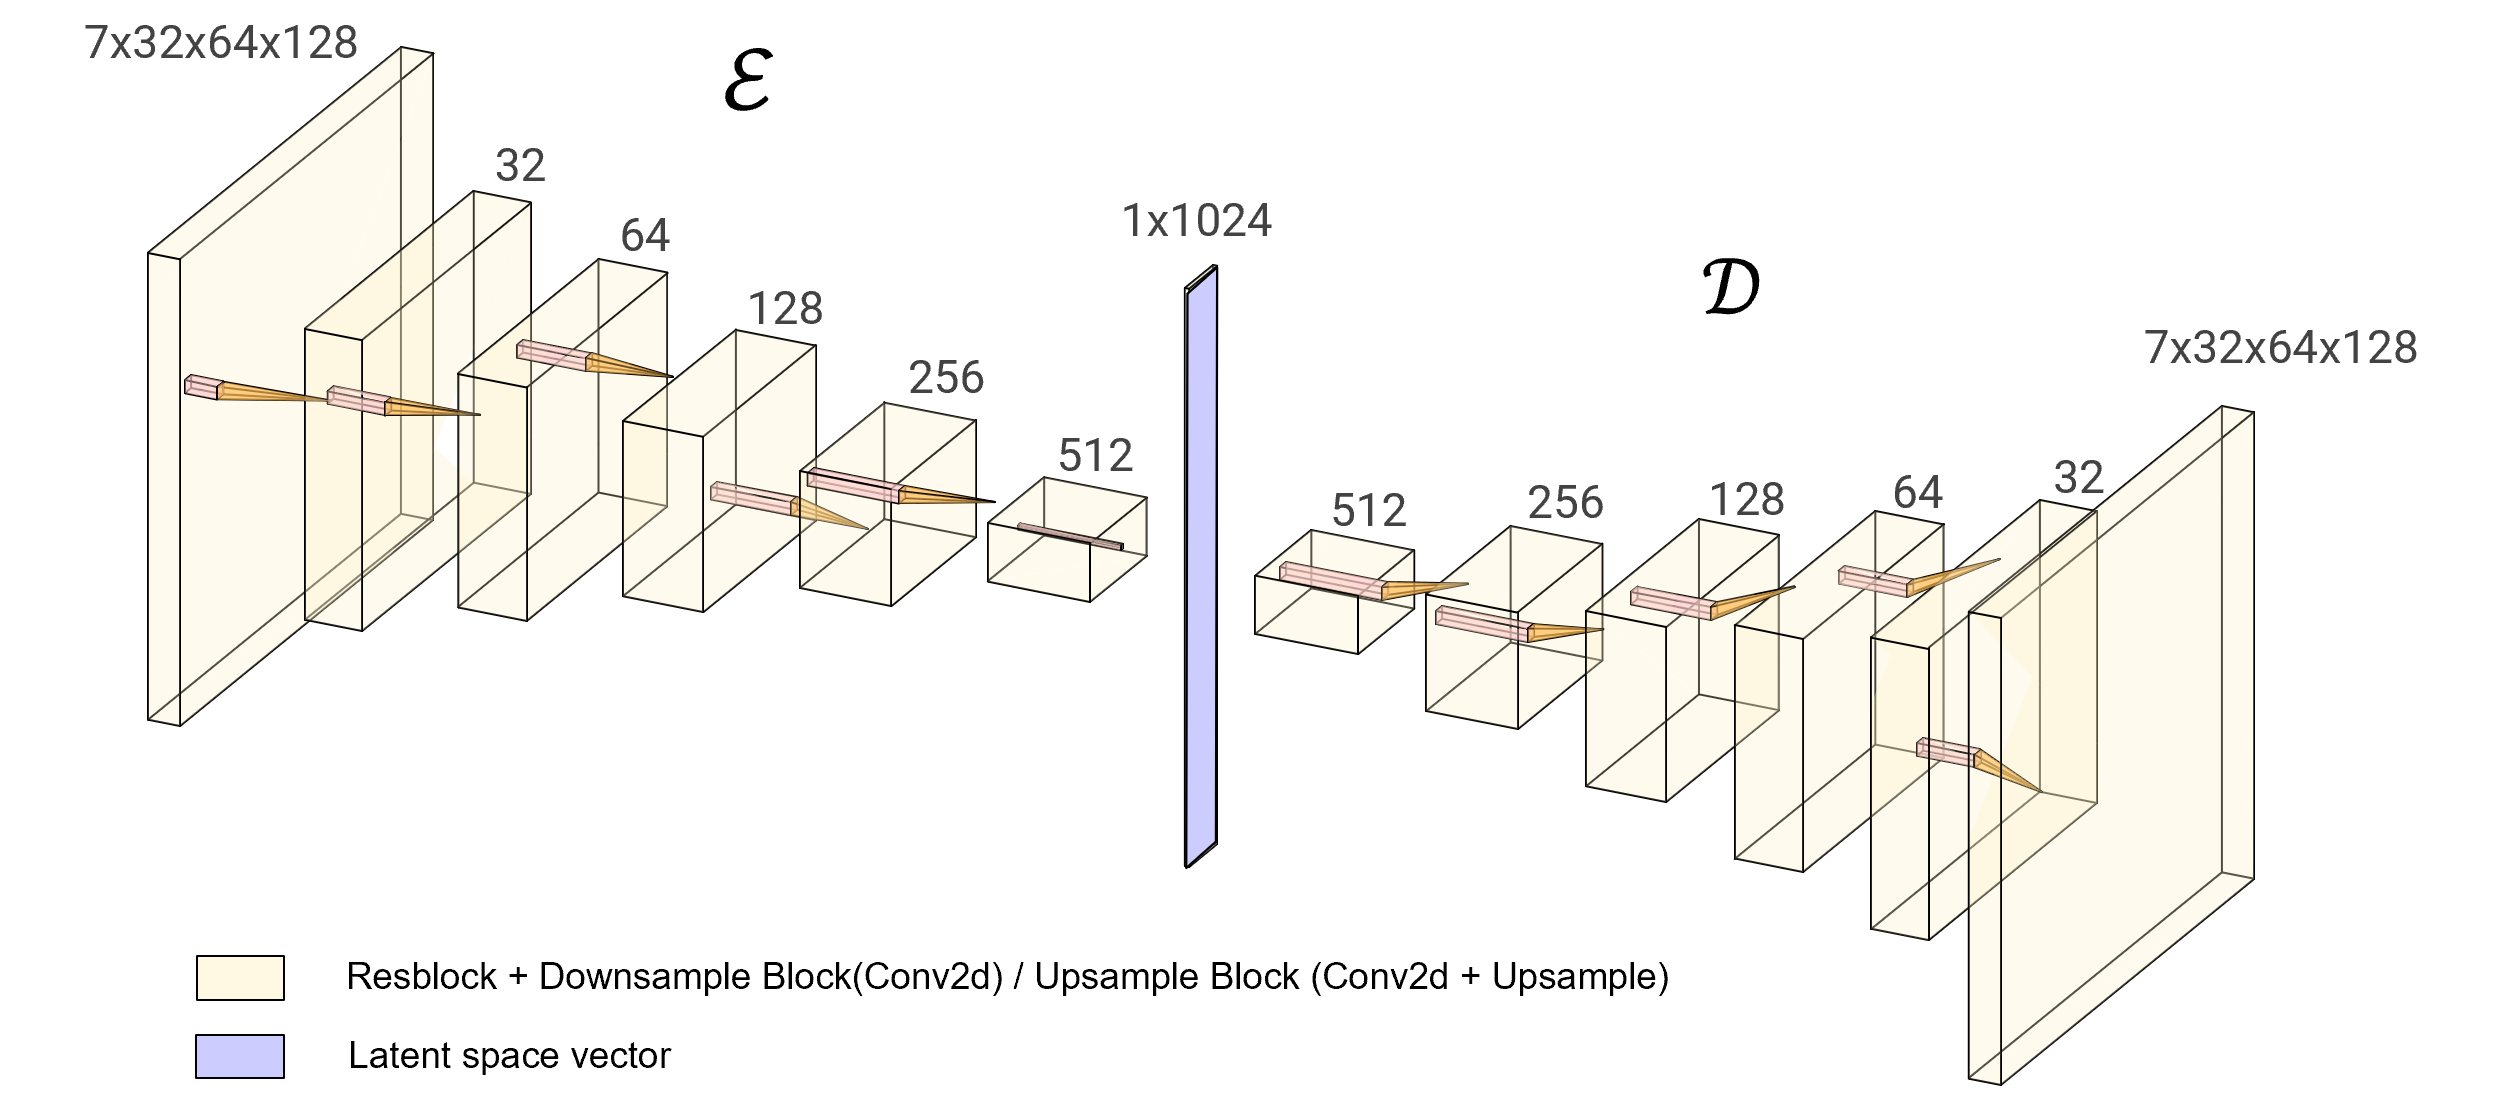
\includegraphics[width=\textwidth]{figures/model_cae.png}
        \caption{Reduced-order model: frame-wise CAE architecture.}
        \label{fig:cae}
    \end{subfigure} \\[11mm]
    \begin{subfigure}[t]{0.75\textwidth}
        \centering
        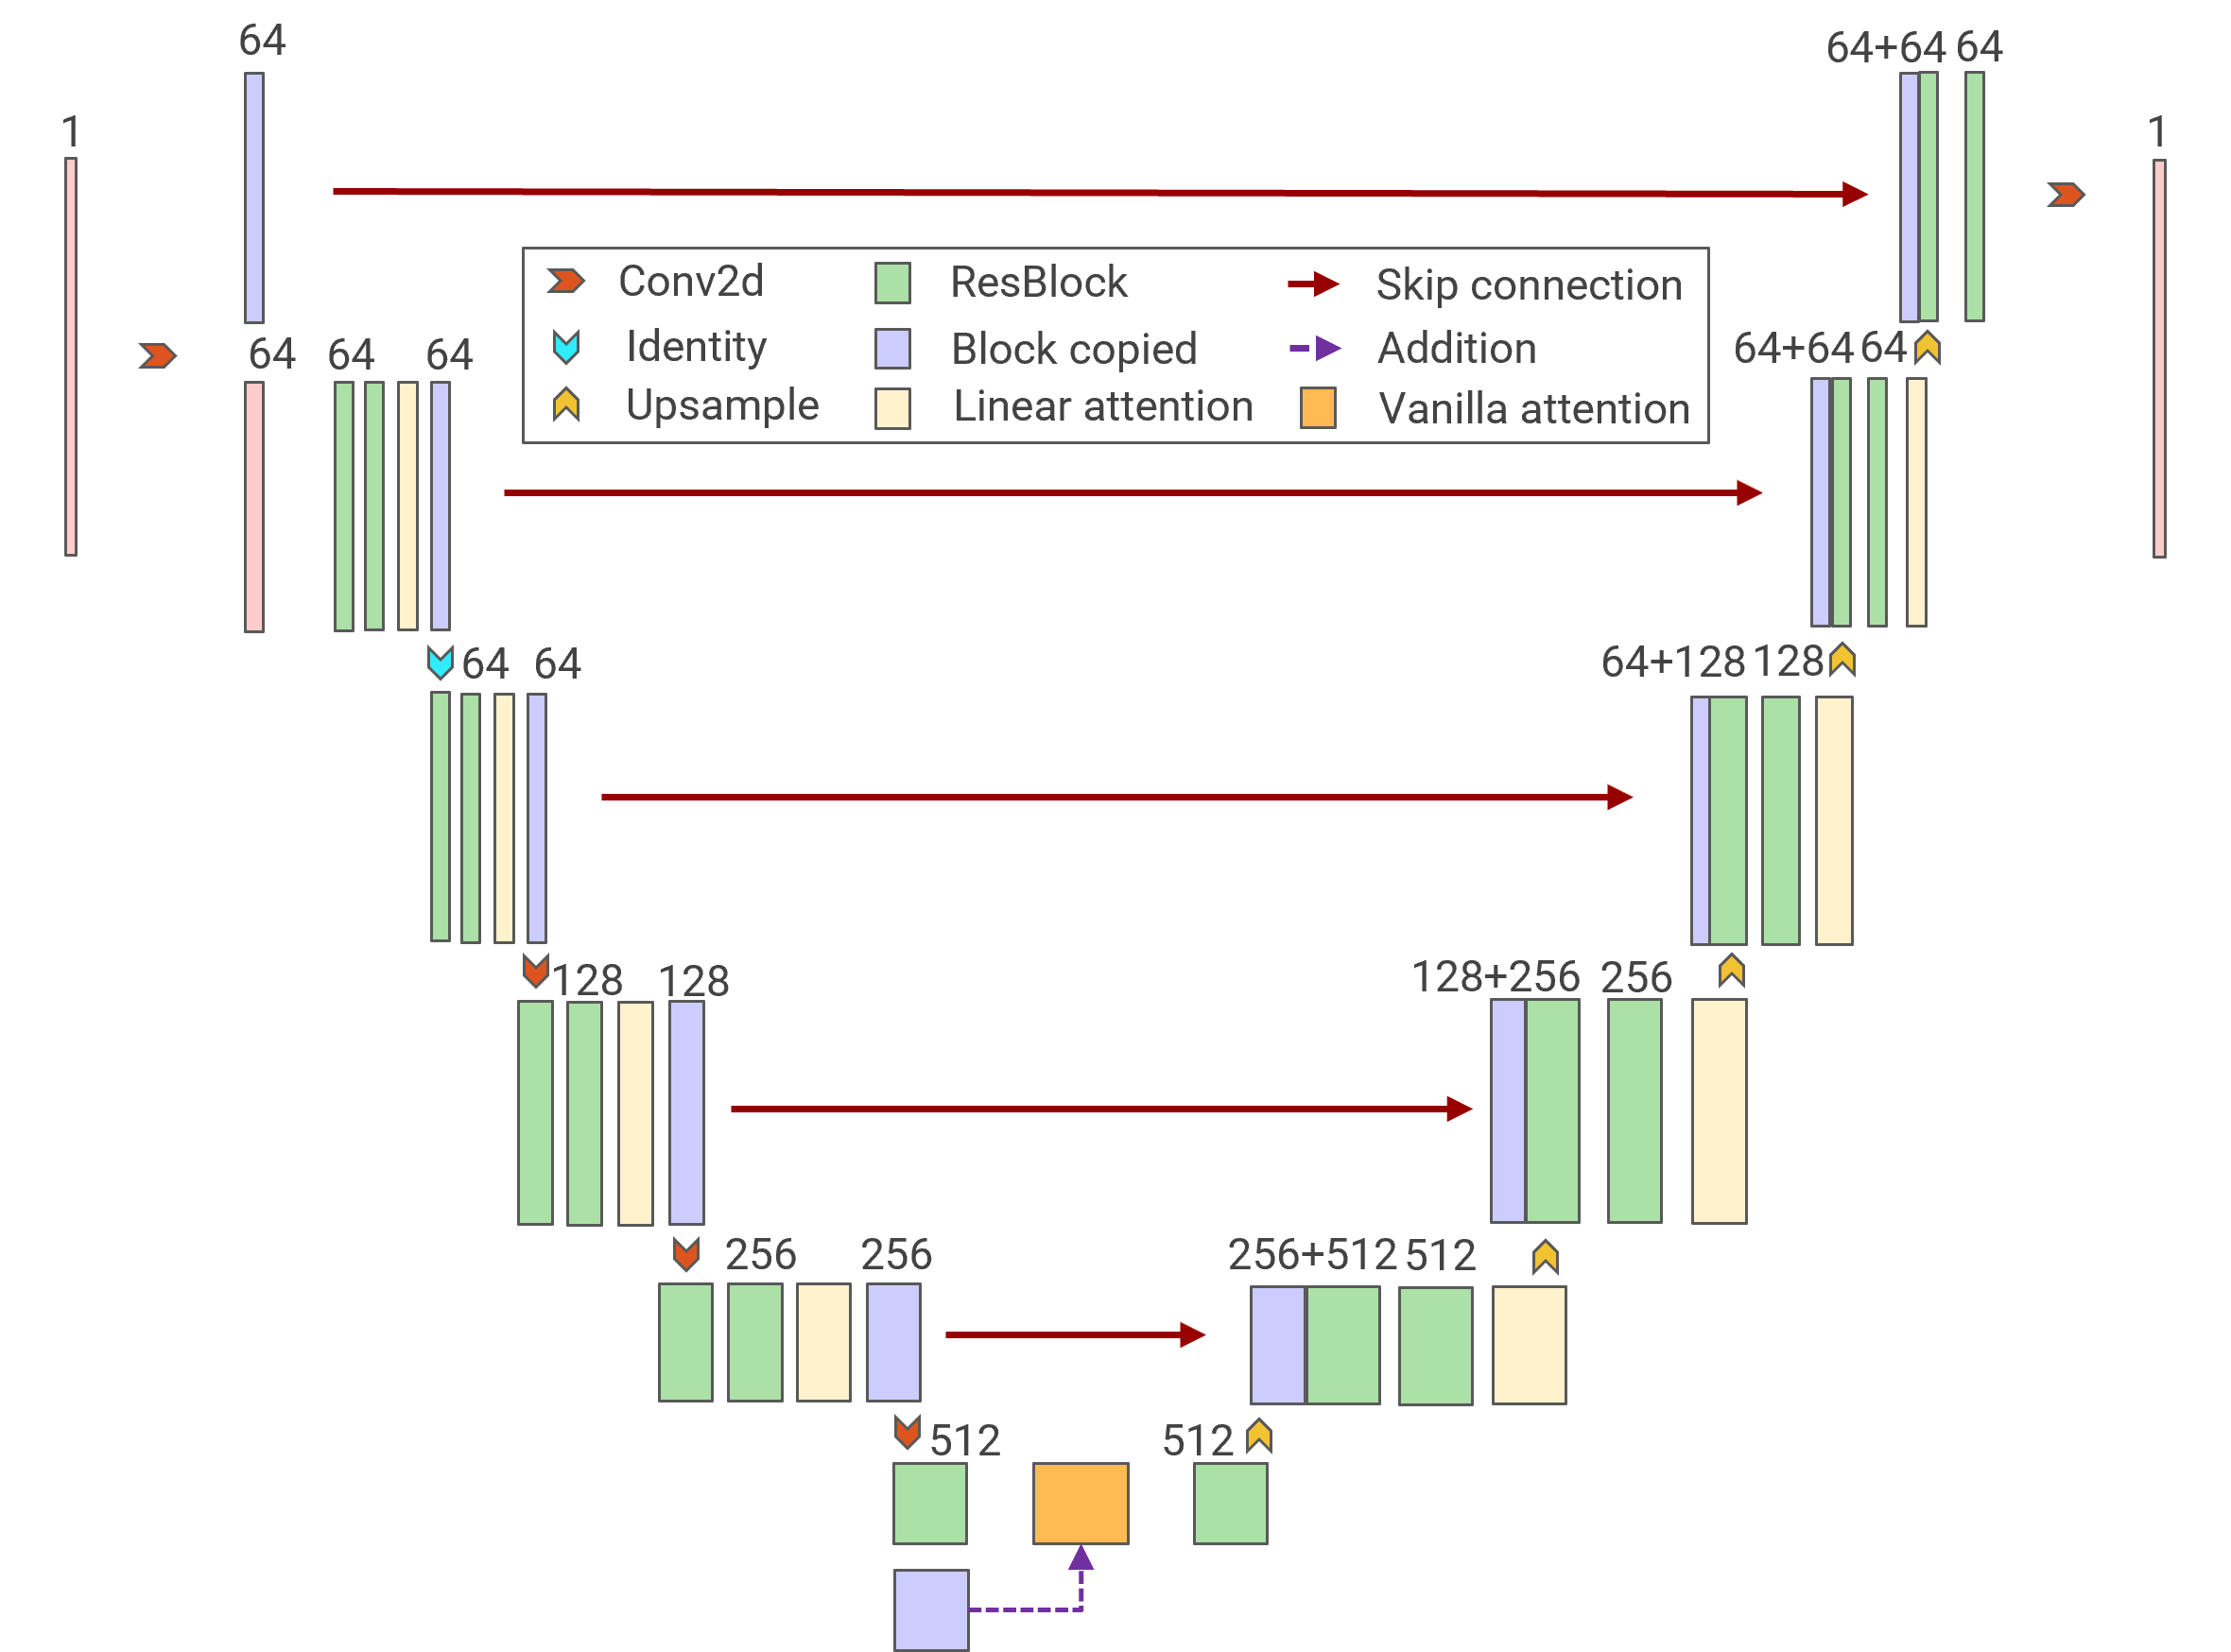
\includegraphics[width=\textwidth]{figures/model_unet.png}
        \caption{The backbone UNet architecture in LDM.}
        \label{fig:unet}
    \end{subfigure} \\[5mm]
    \caption{Overview of the implemented model architectures in this project.}
\end{figure}
\clearpage

\section{Other prediction results}
\begin{figure}[htbp]
    \renewcommand{\figurename}{Figure}
    \renewcommand{\thefigure}{B2}
    \centering
    \begin{subfigure}[t]{0.99\textwidth}
        \centering
        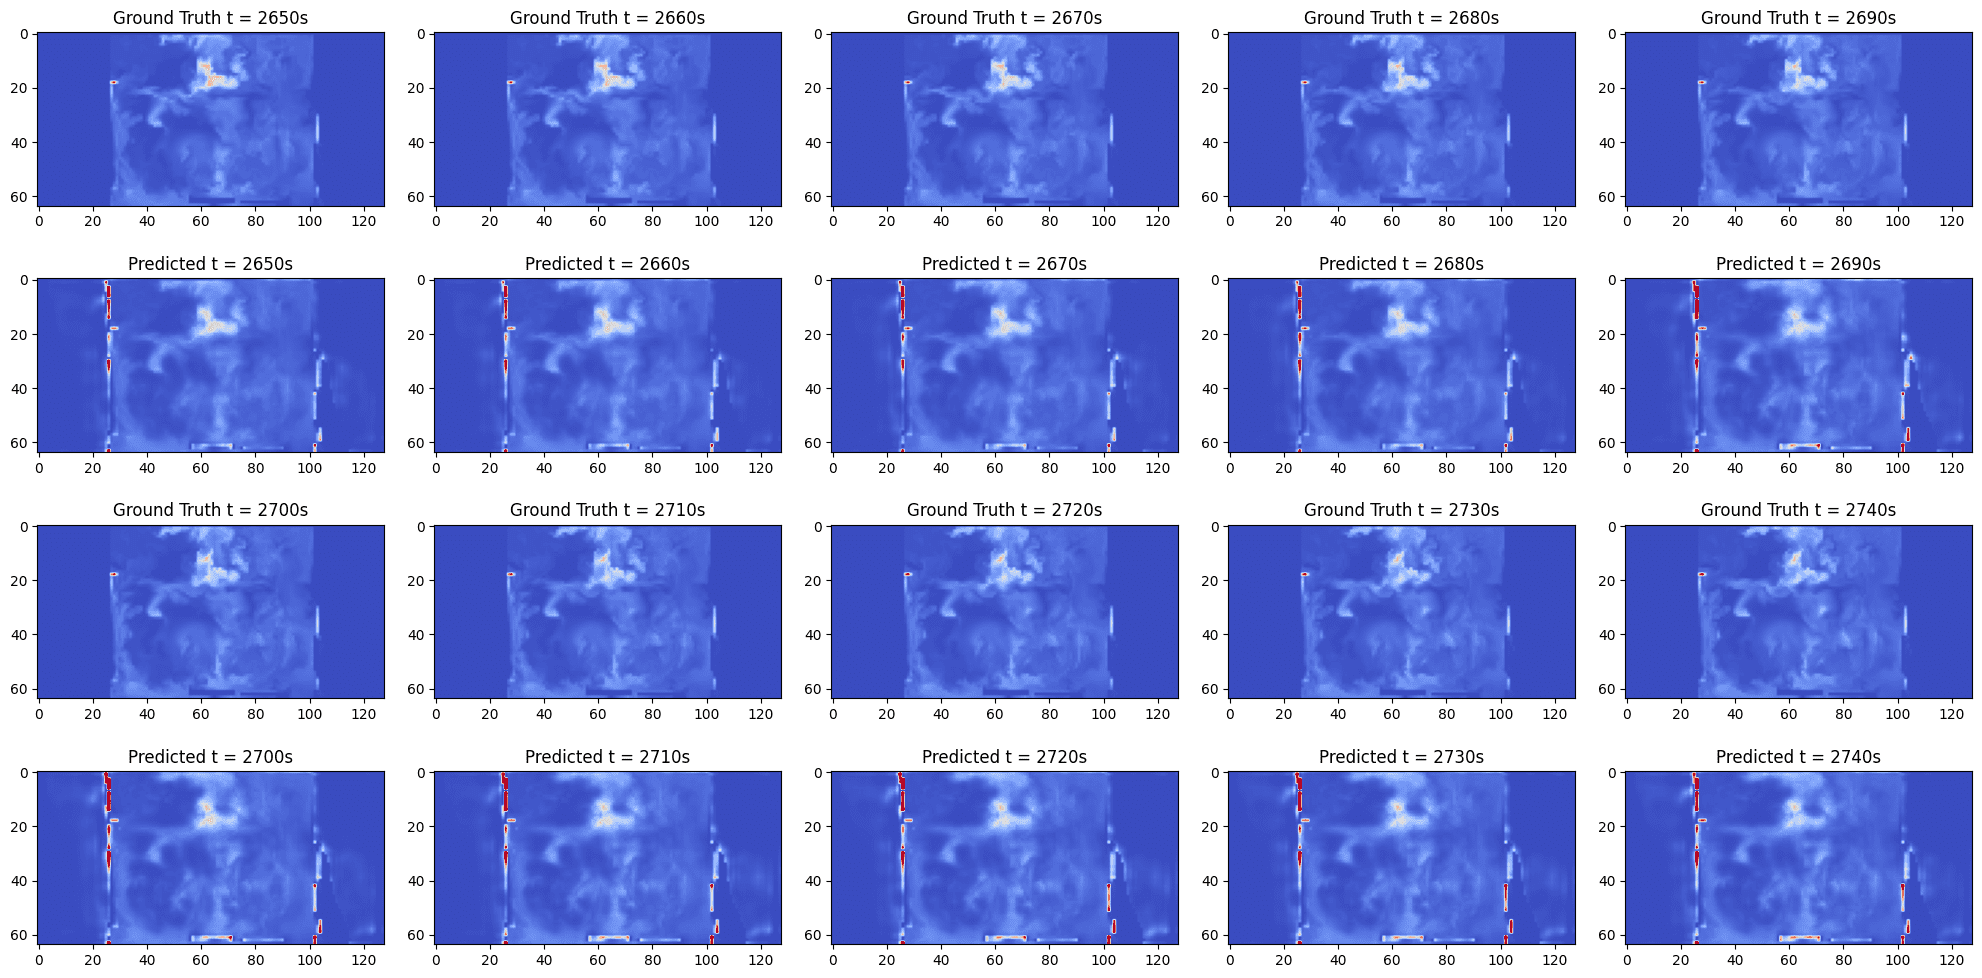
\includegraphics[width=\textwidth]{figures/co2_10_2650.png}
        \caption{CO2 Tracer predictions for the next 10 time steps $t \in [2650s, 2740s]$.}
        \label{fig:co2_10_2650}
    \end{subfigure} \\[6mm]
    \begin{subfigure}[t]{0.99\textwidth}
        \centering
        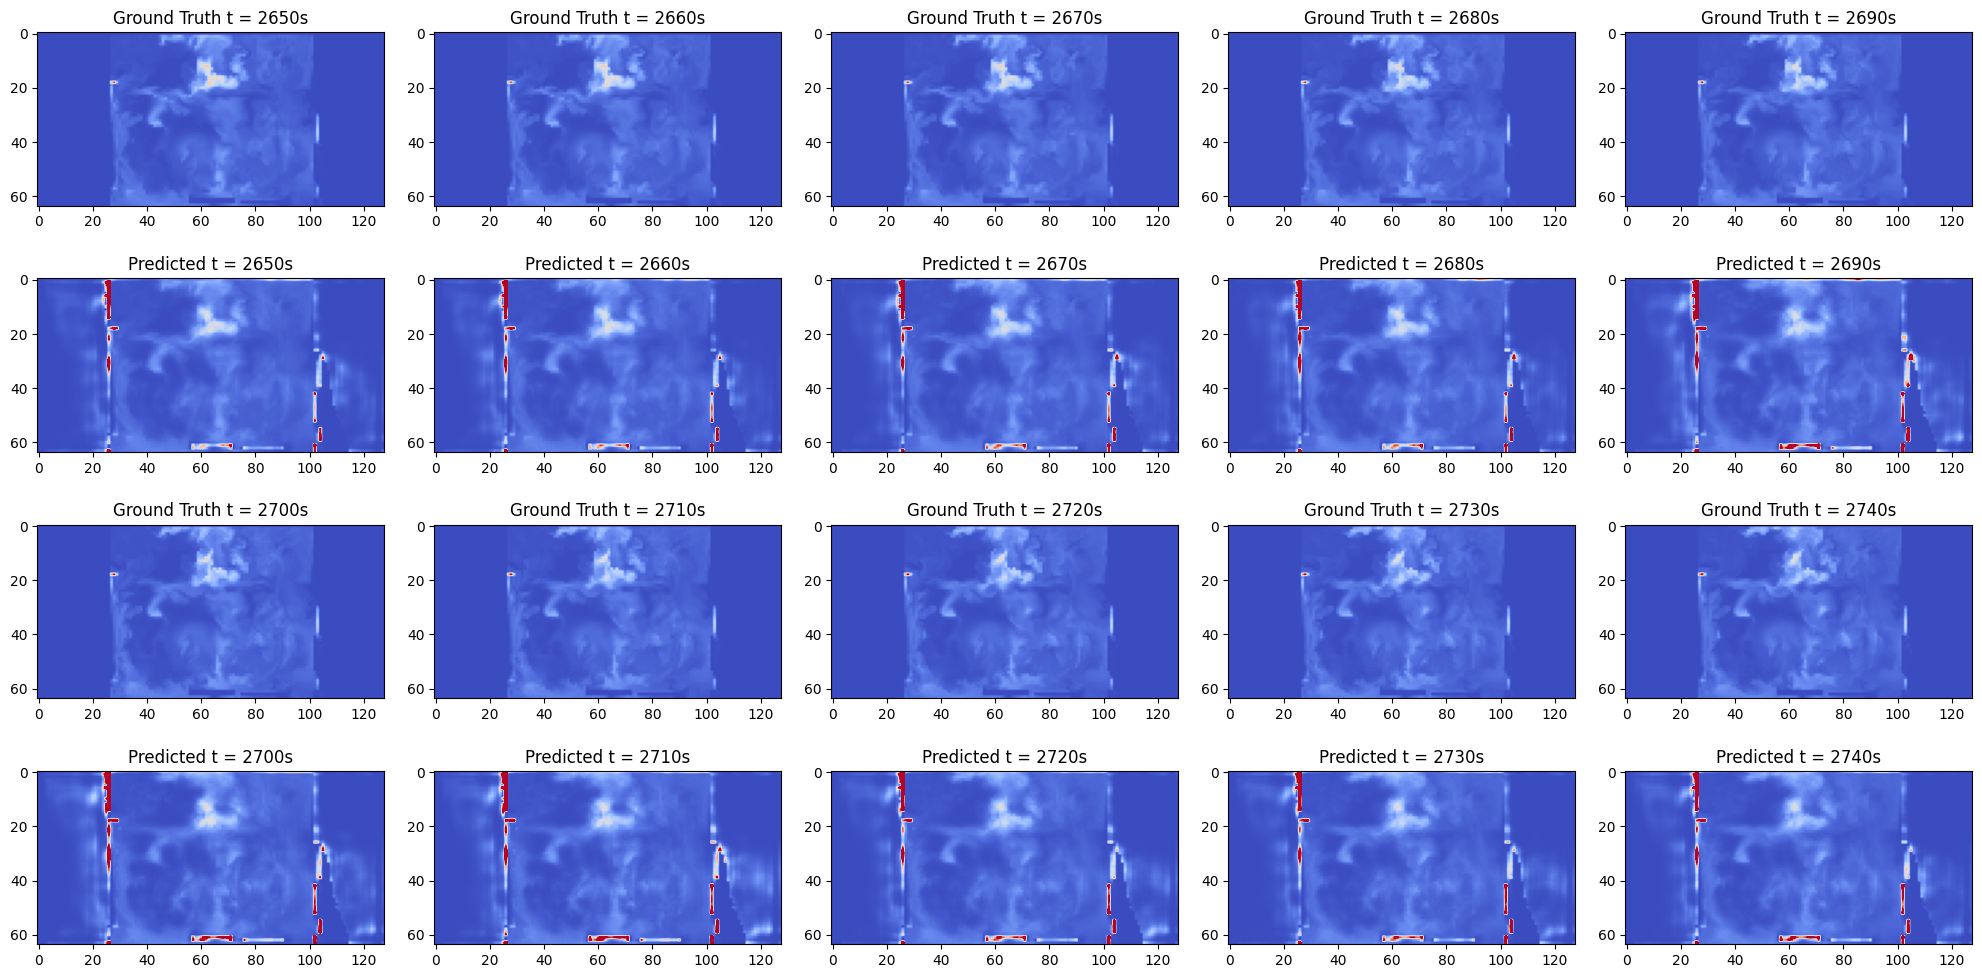
\includegraphics[width=\textwidth]{figures/humid_10_2650.png}
        \label{fig:humid_10_2650}
        \caption{Humidity predictions for the next 10 time steps $t \in [2650s, 2740s]$.}
    \end{subfigure}
    \caption{Other prediction results of xy-slice at z\_idx=16 for the fields 'CO2' and 'Humidity' for time step $t \in [2650s, 2740s]$ in the training set.}
    \label{fig:other_preds}
\end{figure}

\clearpage

\begin{figure}[htbp]
    \renewcommand{\figurename}{Figure}
    \renewcommand{\thefigure}{B3}
    \centering
    \begin{subfigure}[t]{0.99\textwidth}
        \centering
        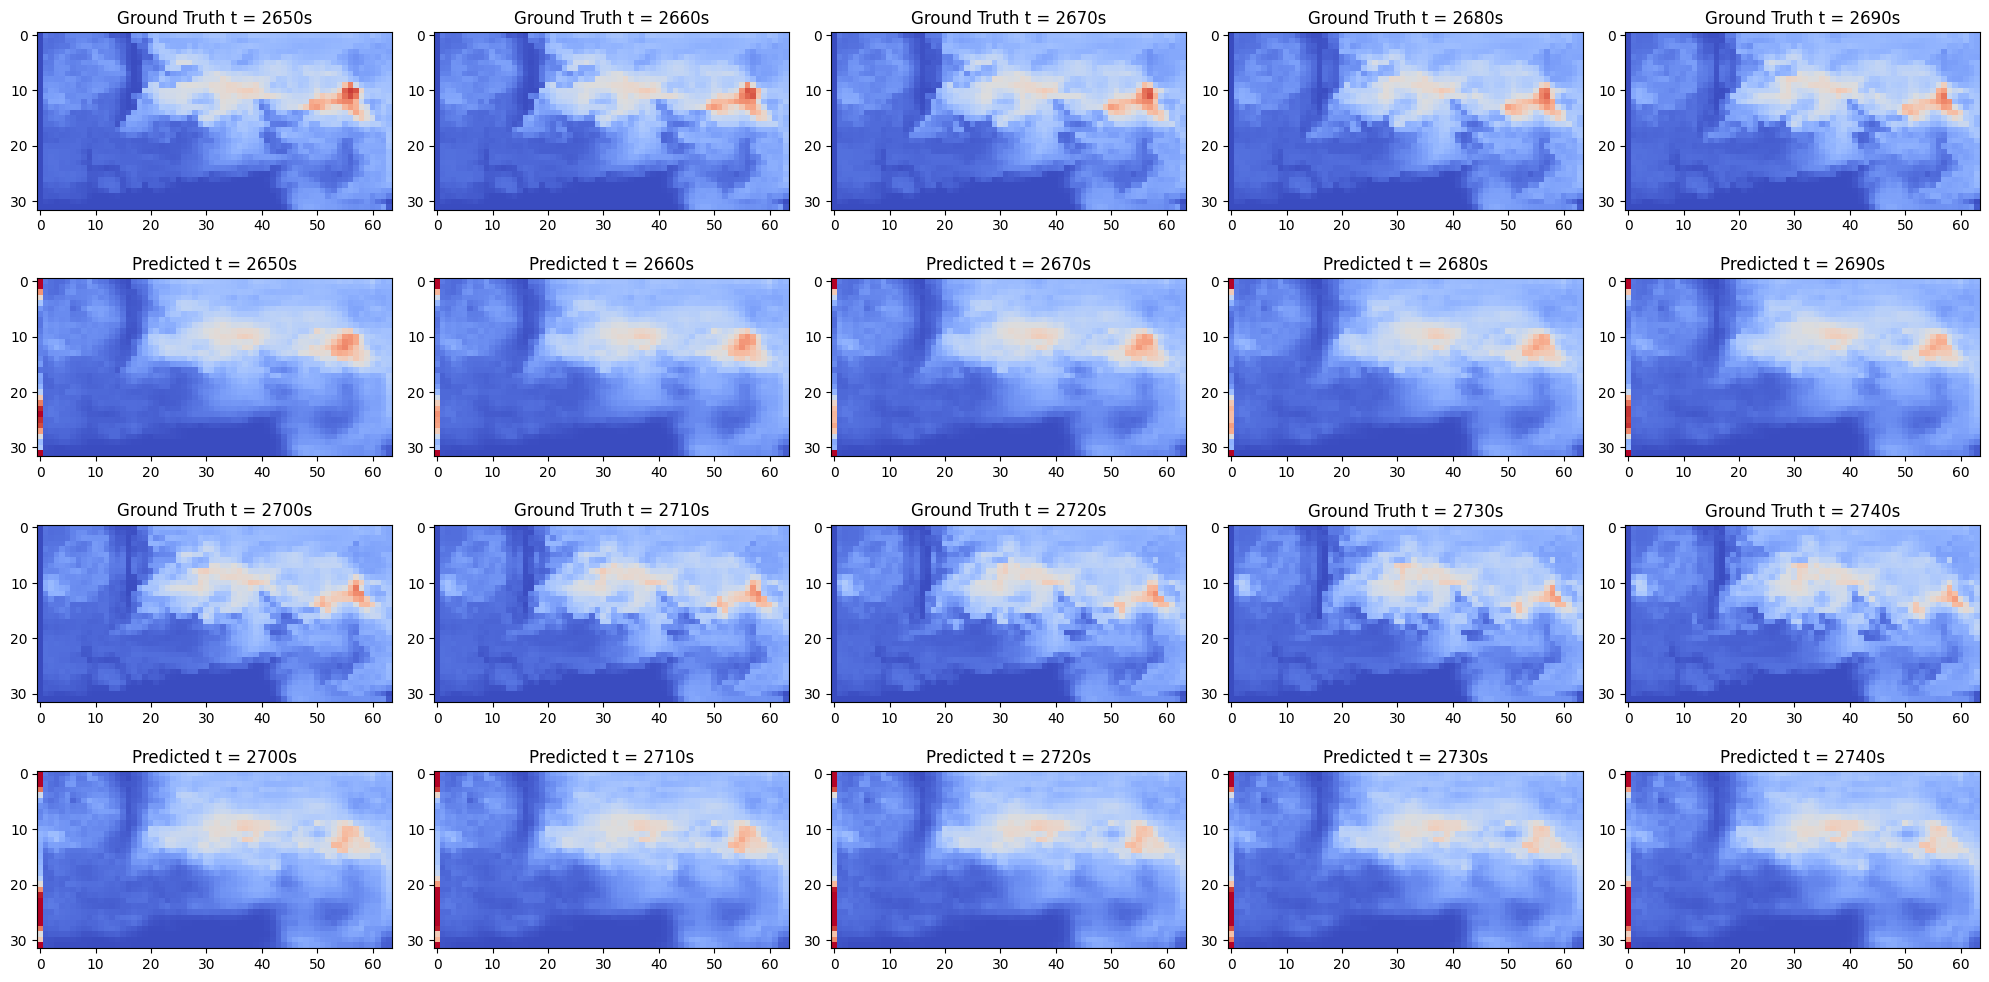
\includegraphics[width=\textwidth]{figures/co2_10_2650_yidx.png}
        \caption{CO2 Tracer predictions for the next 10 time steps $t \in [2650s, 2740s]$ of xz-slice at y\_idx=32.}
        \label{fig:co2_10_2650_xz}
    \end{subfigure} \\[5mm]
    \begin{subfigure}[t]{0.99\textwidth}
        \centering
        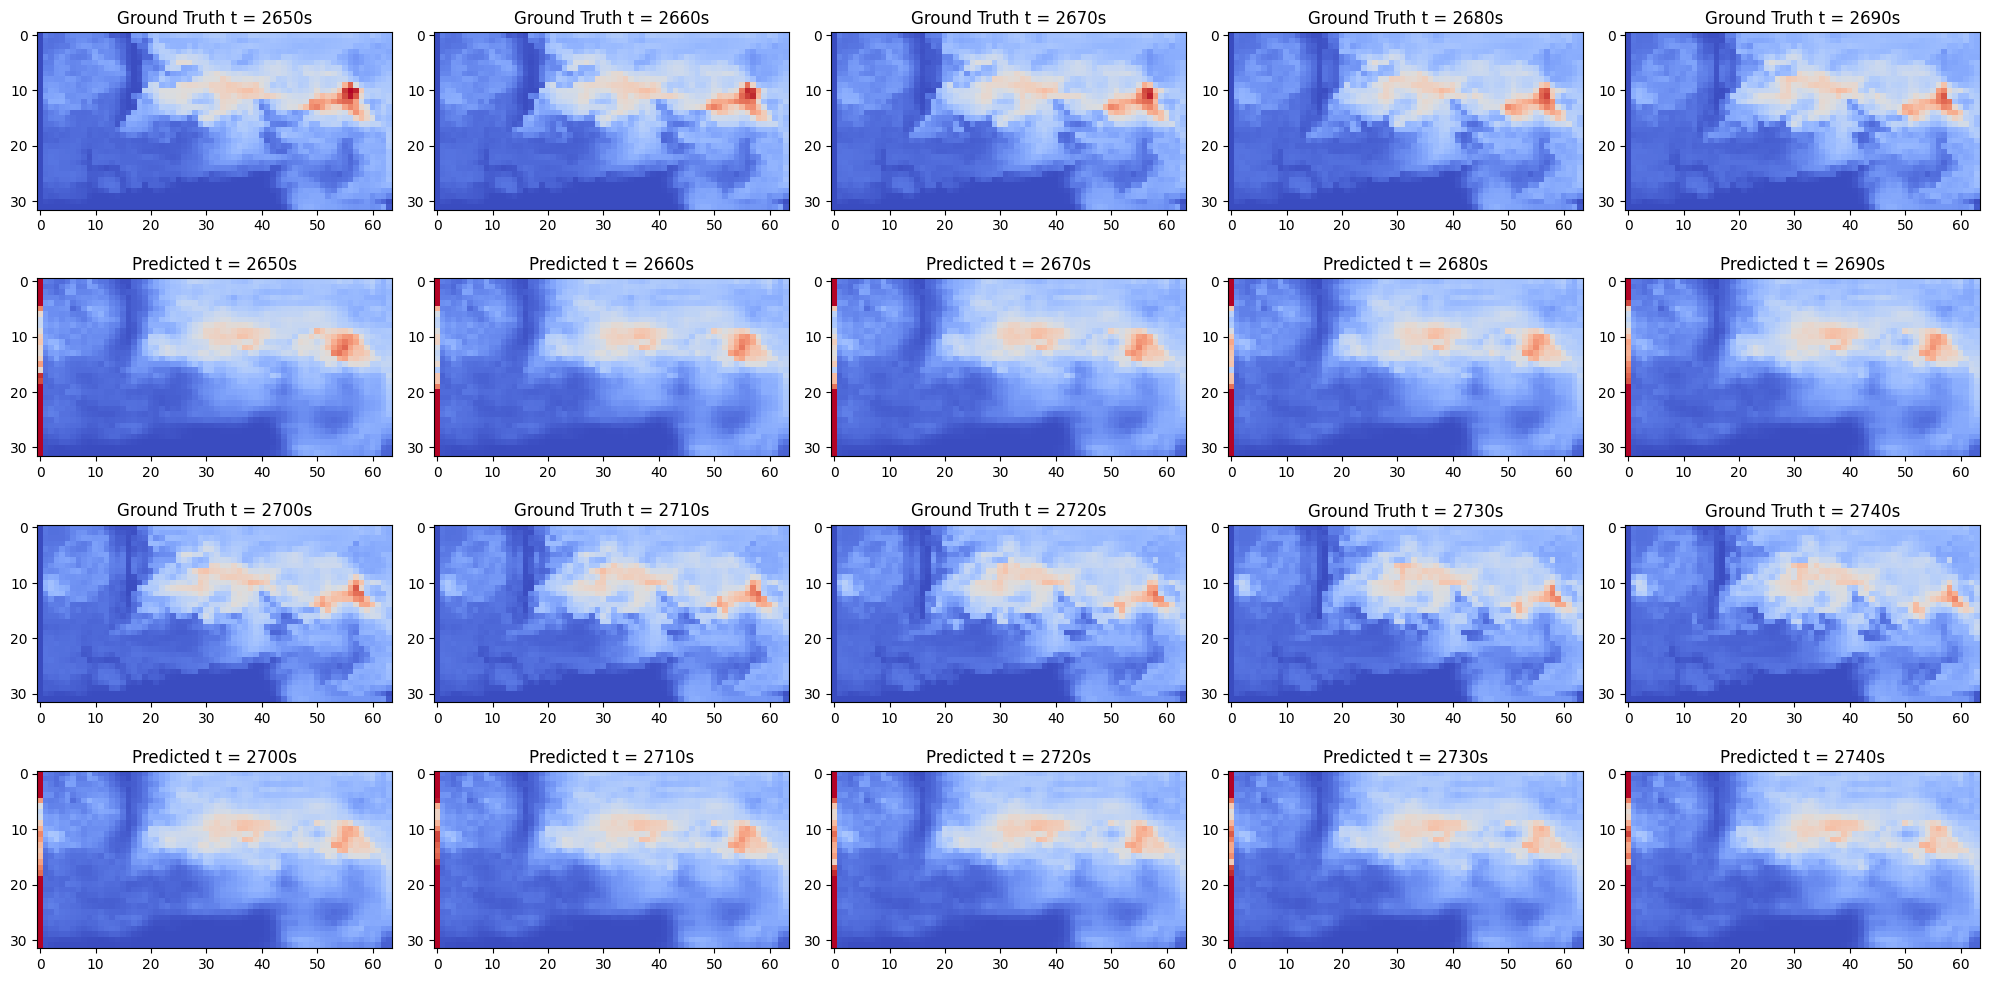
\includegraphics[width=\textwidth]{figures/humid_10_2650_yidx.png}
        \label{fig:humid_10_2650_xz}
        \caption{Humidity predictions for the next 10 time steps $t \in [2650s, 2740s]$ of xz-slice at y\_idx=32.}
    \end{subfigure}
    \caption{Prediction results of other slices (xz-slice at y\_idx=32) for the four fields: 'CO2', 'Humidity', 'Temperature', and 'Vx' for time step $t \in [2650s, 2740s]$.}
    \label{fig:other_preds_xy}
\end{figure}

\clearpage

\begin{figure}[htbpt] \ContinuedFloat
    \renewcommand{\figurename}{Figure}
    \renewcommand{\thefigure}{B3}
    \begin{subfigure}[t]{0.99\textwidth}
        \centering
        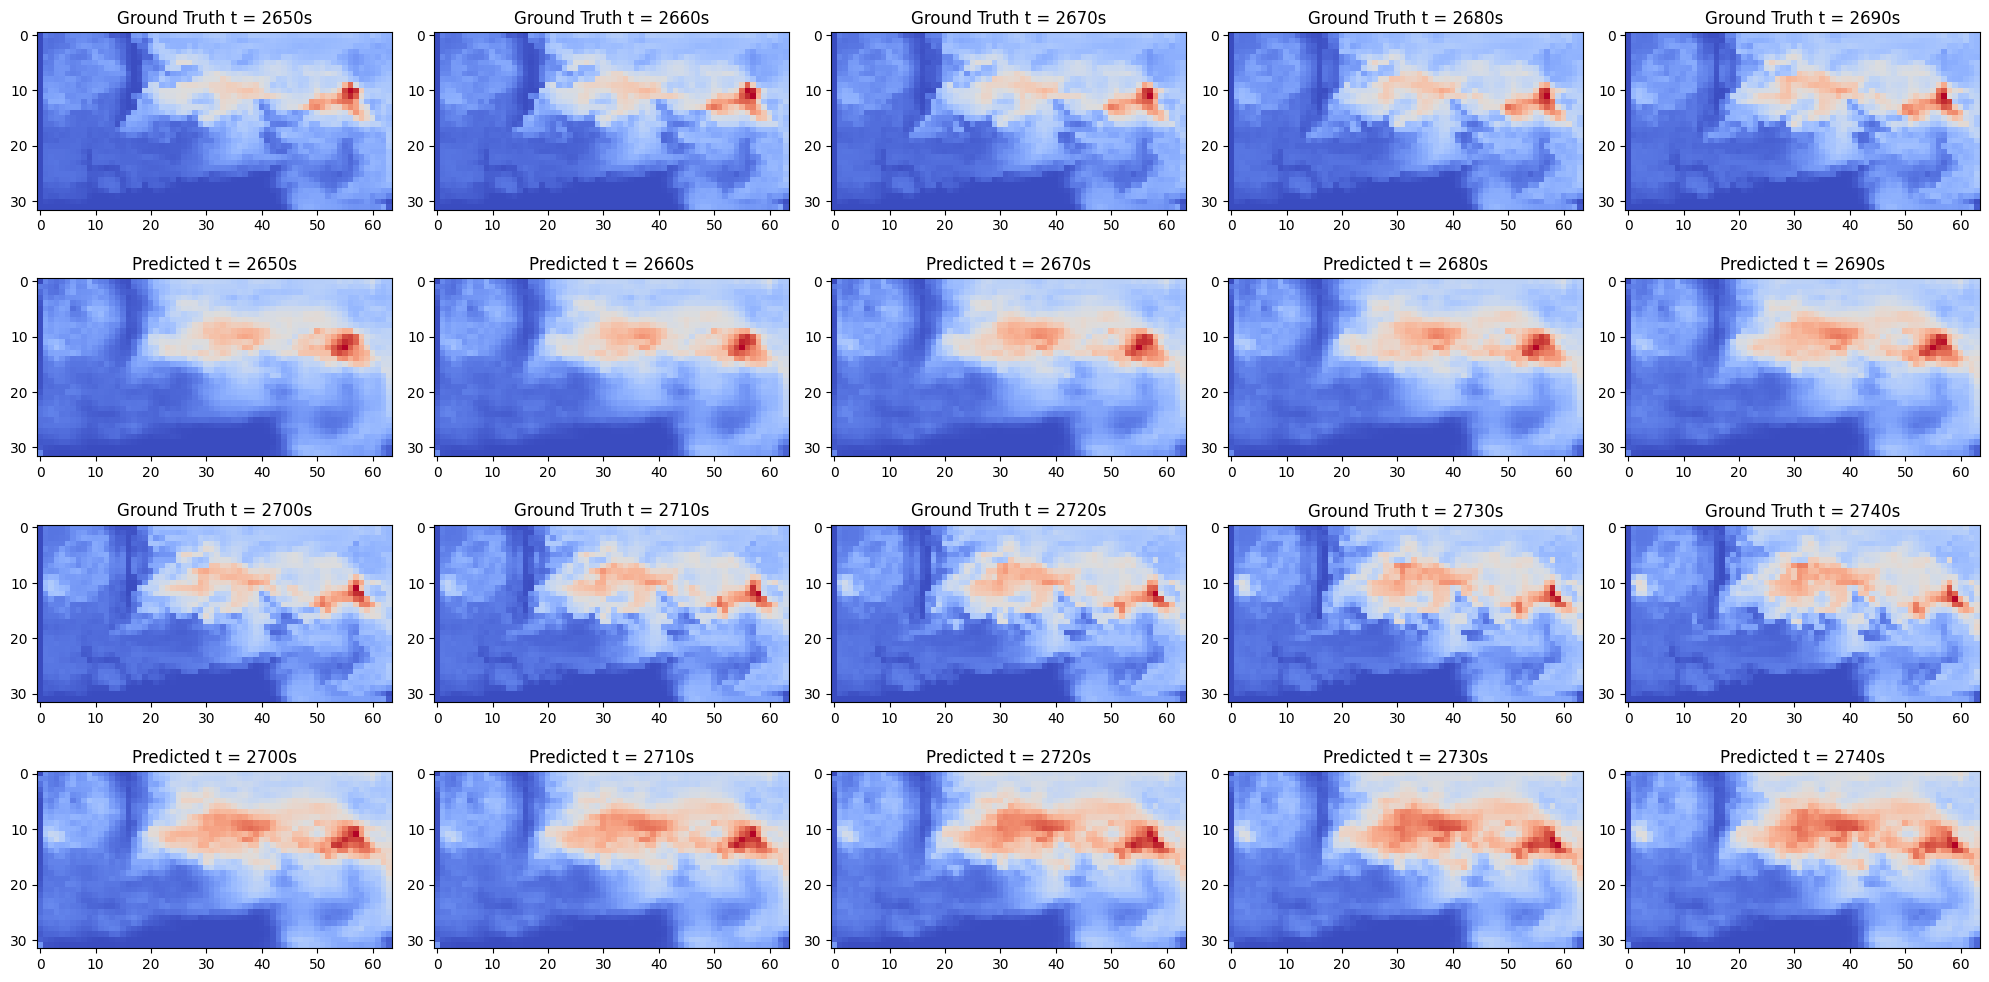
\includegraphics[width=\textwidth]{figures/temp_10_2650_yidx.png}
        \caption{Temperature predictions for the next 10 time steps $t \in [2650s, 2740s]$ of xz-slice at y\_idx=32.}
        \label{fig:temp_10_2650_xz}
    \end{subfigure} \\[10mm]
    \begin{subfigure}[t]{0.99\textwidth}
        \centering
        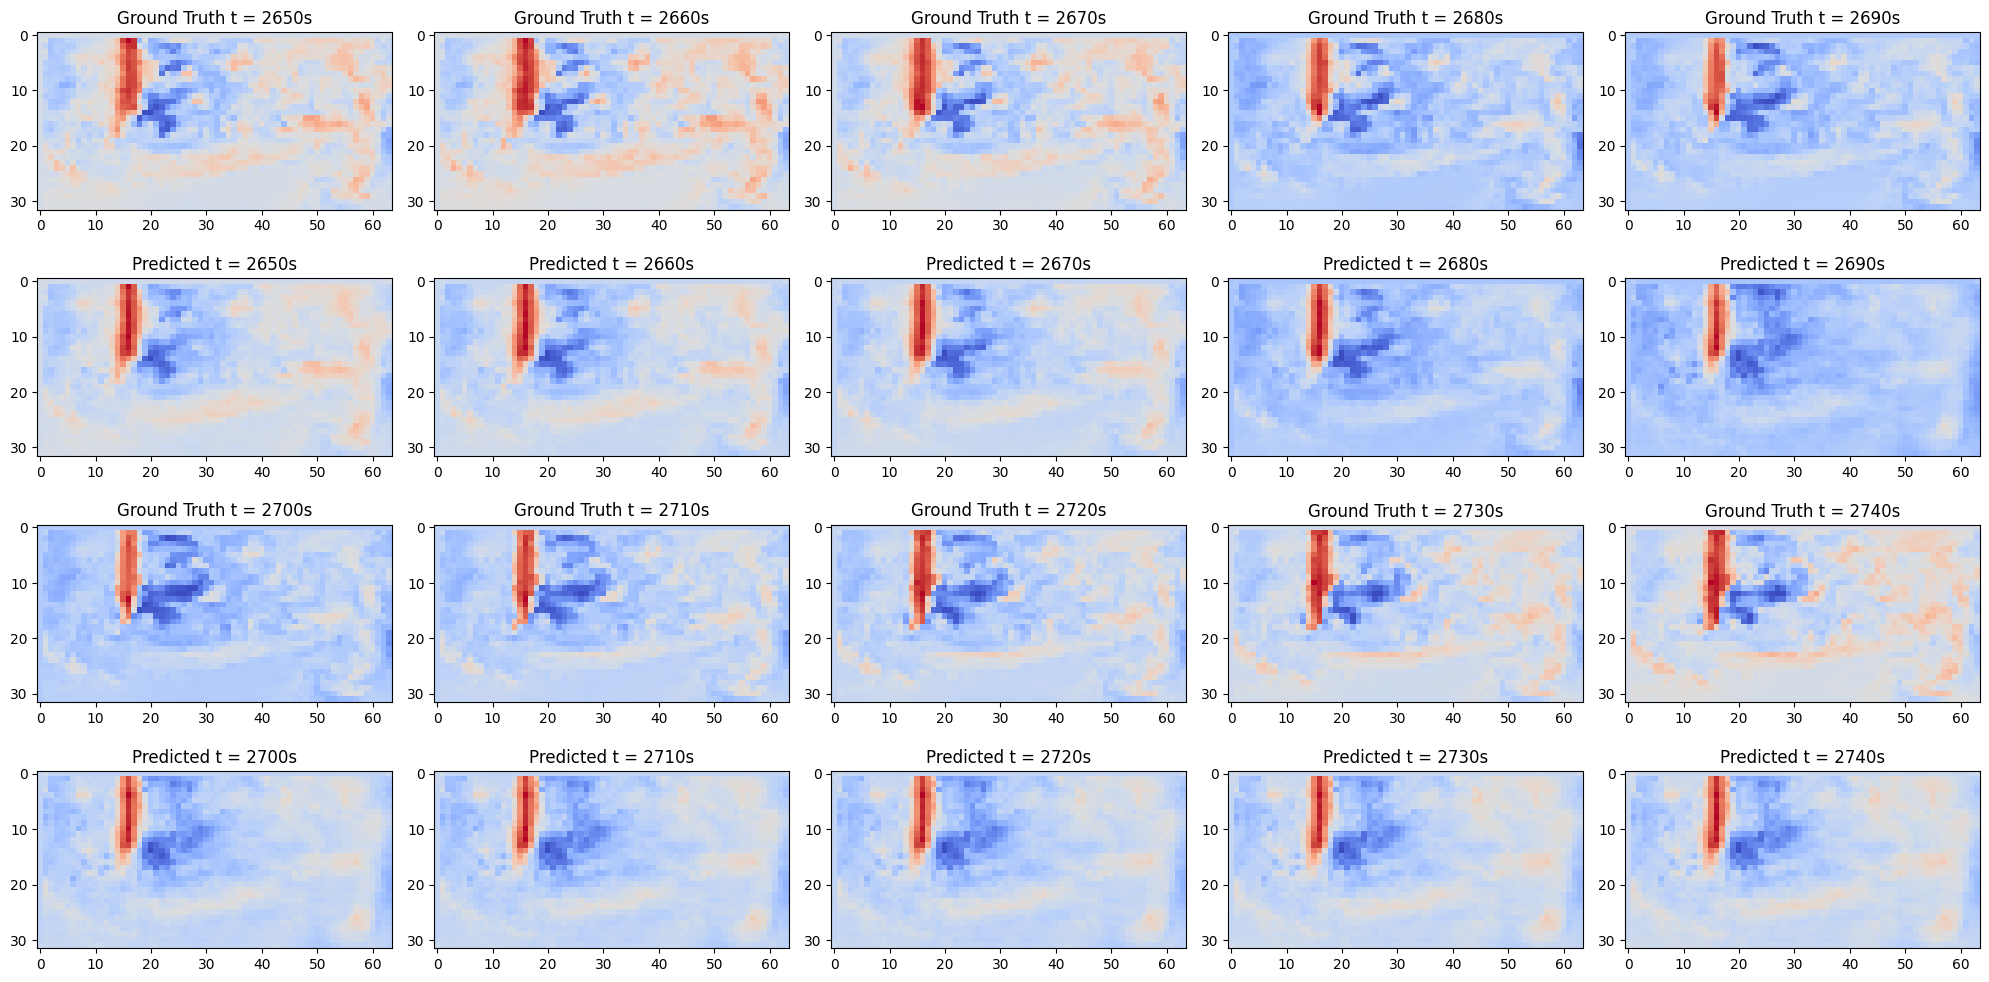
\includegraphics[width=\textwidth]{figures/vx_10_2650_yidx.png}
        \caption{Vx predictions for the next 10 time steps $t \in [2650s, 2740s]$ of xz-slice at y\_idx=32.}
        \label{fig:vx_10_2650_xz}
    \end{subfigure}
    \label{fig:other_preds_xy_2}
    \caption{Prediction results of other slices (xz-slice at y\_idx=32) for the four fields: 'CO2', 'Humidity', 'Temperature', and 'Vx' for time step $t \in [2650s, 2740s]$.}
\end{figure}
%TC:endignore
\end{document}
